\documentclass{aastex63}
\usepackage{amsmath}
\newcommand{\be}{\begin{eqnarray}}
\newcommand{\ee}{\end{eqnarray}}
\def\la{\mathbin{\lower 3pt\hbox
      {$\rlap{\raise 5pt\hbox{$\char'074$}}\mathchar"7218$}}}
\def\ga{\mathbin{\lower 3pt\hbox
      {$\rlap{\raise 5pt\hbox{$\char'076$}}\mathchar"7218$}}} %> or of order
\renewcommand{\vec}[1]{\mathbf{#1}}
\newcommand{\grad}{\mathbf{\nabla}}
\newcommand\lya{Ly$\alpha$\ }


\received{}
\revised{}
\accepted{\today}
\submitjournal{APJ}


\shorttitle{Resonant Scattering of \lya}
\shortauthors{McClellan et al.}

\graphicspath{{./}{figures/}}


\begin{document}

\title{Resonant Scattering in a Uniform Sphere with Large Optical Depth}



\correspondingauthor{B. Connor McClellan}
\email{bcm2vn@virginia.edu}

\author[0000-0002-6040-8281]{B. Connor McClellan}
\author[0000-0001-7488-4468]{Shane Davis}
\author[0000-0001-5611-1349]{Phil Arras}
\affiliation{Department of Astronomy, University of Virginia, Charlottesville, VA 22904, USA}


\begin{abstract}

The radiation transfer equation for resonant scattering is solved in spherical geometry. A monochromatic source of photons is assumed at the center of a uniform sphere of constant gas density. The intensity within the sphere and at its surface is found in the limit of large line-center optical depth using the Eddington approximation for the angular dependence. Two limits are studied: a steady source and an impulsive source. For the steady-state problem, the solution can be represented as a sum of two terms: a previously-known analytic solution of the equation with  mean intensity $J=0$ at the surface, and a novel, semi-analytic solution which enforces the correct boundary condition of zero-ingoing intensity at the surface. This solution is compared to that of the Monte-Carlo method, which is valid at arbitrary optical depth. It is shown that the size of the correction is order unity when the spectral peaks approach the Doppler core and decreases slowly with line center optical depth, which may explain discrepancies in previous studies. For the impulsive problem, the time, spatial, and frequency dependence of the solution are expressed using an eigenfunction expansion in order to characterize the escape time distribution and emergent spectra of photons. It is shown that the lowest-order eigenfrequency agrees well with the decay rate found in the Monte Carlo escape time distribution at sufficiently large line-center optical depths.

\end{abstract}


\keywords{}

\section{Introduction}
\label{sec:intro}

The outer layers of the atmosphere are central to a planet's evolution, since they can shelter the lower atmosphere from high energy radiation as well as regulate the escape of gas into space. Given the abundance of hydrogen and its large cross section, the Lyman $\alpha$ (Ly$\alpha$) line is an important component of the radiation field. There are two sources of Ly$\alpha$: the star, and recombinations in the planet's atmosphere. \lya may ionize atoms and dissociate molecules, as well as exert pressure forces that drive an outflow. \lya can also excite H atoms to the 2p state, creating a population of Balmer-line absorbers that can be observed via transmission spectroscopy \citep{2017ApJ...851..150H}. Due to the low gas densities in the upper atmosphere, collisional de-excitation and broadening are of secondary importance and \lya may undergo ``resonant scattering''.

Hubble Space Telescope (HST) observations with the STIS have found large \lya transit depths around a handful of exoplanets \citep{2003Natur.422..143V, 2012A&A...543L...4L, 2012A&A...547A..18E, 2015Natur.522..459E,  2017A&A...597A..26B, 2017A&A...599L...3B, 2017A&A...602A.106B, 2018A&A...620A.147B, 2019AJ....158...50W, 2019EPSC...13.1928L, 2020ApJ...888L..21G,2021arXiv210309864B}. These observations have revealed a population of atoms extending out to distances of order a few planetary radii or more for several planets around bright, nearby stars, motivating a study of the physics of \lya interactions with the H atom population. The transition from the atomic to the molecular layer in these hot upper atmospheres may take place at pressures of order ${\sim}\ 10\ \mu$bar (see discussion in \citet{2017ApJ...851..150H} for details). This suggests the presence of a thick layer of atomic H which can have a line center optical depth of $\tau_0\ {\sim}\ 10^8$. A careful treatment of resonant scattering is necessary in order to construct accurate models of H atom excitation, heating, and radiative forces. 

Due to the technical challenge of including resonant scattering, the fully three-dimensional geometry, and the presence of an outflow, numerical simulations may be required to fully understand the dynamics of these irradiated exoplanet atmospheres. The large optical depths at \lya line center impose a steep computational cost for solving radiative transfer with Monte Carlo methods directly coupled with fluid dynamics. The number of scatterings a photon undergoes is proportional to the line center optical depth, $\tau_0$, of the domain.  Near the base of the atomic layer, the line center optical depth is ${\sim}10^8$, so most of the time is spent following photons in these cells. A method that can treat these zones incorporating a direct solution rather than traditional Monte Carlo has the potential to greatly accelerate the calculation.

Approximate analytic solutions for resonant scattering exist in certain limits. \citet{1973MNRAS.162...43H} showed that when most of the radiation is out on the damping wings, the transfer equation reduces to the Poisson equation. However, their solution contains an incorrect treatment of the boundary condition. To our knowledge, the errors introduced by this treatment have never been quantified. They attempt a separation of variables as $J(\tau,\sigma) = \theta(\tau) j(\sigma)$ in spatial variable $\tau$ and frequency variable $\sigma$ (their Equations 16 and 23). The solutions for the eigenfunctions $\theta(\tau)$ and $j(\sigma)$ then depend explicitly on the separation constant $\lambda$. In order to satisfy the boundary conditions, the separation constant is shown to satisfy an eigenvalue equation of the form
\be
\lambda \tan(\lambda B) & = & \frac{3}{2} \phi \Delta,
\label{eq:evalue}
\ee
where $2B$ is the slab optical depth at line center, $\phi$ is the line profile, and $\Delta$ is the Doppler width. The key point is that the line profile depends on one of the coordinates: frequency. This causes the eigenvalues of the separation constant to be frequency-dependent. Thus, the separation ``constant'' is not constant, and the function does not satisfy the Poisson equation since the frequency derivatives will act on the separation ``constant", giving extra terms. In the limit of large optical depth $B$, they approximate the eigenvalues as $\lambda_n B \simeq \pi (n-1/2)$. However, this gives zero mean intensity at the surface. Their Equation 34 subsequently allows $\lambda$ to have a small deviation from the above expression, which is explicitly frequency dependent. This allows a nonzero intensity at the surface, but at the cost of rendering the separation of variables assumption invalid. Our treatment, using the correct boundary condition, quantifies the errors in their ansatz.

Several other works have followed \citet{1973MNRAS.162...43H}, building upon their result without addressing the incorrect boundary condition. \citet{1990ApJ...350..216N} attempts to extend the solution to media of intermediate optical depth, including the effects of scattering in the Doppler core of the line, but again does not use the correct boundary condition. \citet{2006ApJ...649...14D} generalize the same problem to spherical geometry, as is used here.

\section{STEADY-STATE SOLUTION}
\label{sec:steadystate}

Consider a sphere of radius $R$ with uniform density $n_{\rm sc}$, luminosity $L$, and line-center optical depth $\tau_0$ containing a point source of photons. We aim to find the intensity within the sphere as a function of radius and photon frequency. The point source is assumed to be a delta function in space and photon frequency. Photons of frequency $\nu$ near the line center frequency $\nu_0$ are considered. The photon frequency of the source is $\nu_s$. The Doppler width is $\Delta = \nu_0 v_{\rm th}/c$, where $v_{\rm th}=\sqrt{2k_{\rm B}T/m_{\rm H}}$ is the thermal speed of hydrogen atoms of mass $m_{\rm H}$ and temperature $T$, and $c$ is the speed of light. The photon frequency in Doppler widths is $x = (\nu-\nu_0)/\Delta$, and $x_s = (\nu_s - \nu_0)/\Delta$ is the corresponding source frequency. For upper-state de-excitation rate $\Gamma$, the ratio of natural to Doppler broadening is $a=\Gamma/(4\pi \Delta)$. Here $e$ and $m_e$ are the charge and mass of the electron, $f$ is the oscillator strength of the transition, $\mathcal{H}(x,a)$ is the Voigt function, $k = n_{\rm sc} \pi e^2 f/(m_e c)$, and the Voigt line profile is $\phi = \mathcal{H}(x,a)/(\sqrt{\pi} \Delta)$, which is normalized as $\int d\nu\, \phi(\nu) = 1$. The line center optical depth is then $\tau_0 = kR/(\sqrt{\pi}\Delta)$. 

Appendix \ref{app:rteqn_derivation} contains a derivation of the transfer equation for convenience. Starting with the full transfer equation, Eq. \ref{eq:finaleqn}, ignoring photon destruction and including a photon emission term given by Eq. \ref{eq:jem}, the steady-state transfer equation is
\be
\nabla^2 J + \left( \frac{k}{\Delta} \right)^2 \frac{\partial^2 J}{\partial \sigma^2} & = & 
- \frac{ \sqrt{6} kL}{4\pi \Delta^2} \delta^3(\vec{x} - \vec{x}_s) \delta (\sigma - \sigma_{\rm s}).
\label{eq:rt_no_destr}
\ee
where $J$ is the mean intensity, the spatial variable is $\vec{x}$, and $\vec{x}_s$ is the position of the source.  Following \citet{1973MNRAS.162...43H}, we have used a change of variables from $x$ to $\sigma$,
\be \label{eq:int_change_of_variables}
\sigma(x) = \sqrt{\frac{2}{3}}\int_0^x \frac{dx}{\phi(x) \Delta} \approx \sqrt{\frac{2}{3}}\frac{\pi}{a}\frac{x^3}{3}, 
\ee
where the approximation is applicable on the damping wing. The line profile is then approximately (Equation \ref{eq:app:line_profile_wing})
\be \label{eq:line_profile_approx}
\phi \approx \frac{a}{\pi x^2 \Delta} \approx \frac{1}{3 \Delta}\left(\frac{2a}{\pi}\right)^{1/3}|\sigma|^{-2/3}.
\ee
In Equation \ref{eq:rt_no_destr}, $\sigma_s \equiv \sigma(x_s)$ is the photon frequency of the source. $\sigma_s$ is interchangeable with $x_s$ and $\nu_s$ in Doppler widths or Hz, respectively. Balancing the two terms on the left hand side of Equation \ref{eq:rt_no_destr} gives $\sigma \ {\sim}\ \tau_0$, or $x_{\rm peak}\ {\sim}\ (a\tau_0)^{1/3}$. The boundary condition of no incoming intensity at the surface \citep{1986rpa..book.....R} is
\be
J & = & \sqrt{3} H
\label{eq:bc}
\ee
at $r=R$. 

A solution for the mean intensity $J_d$ which is divergent at $\vec{x}=\vec{x_s}=0$ %TODO: This ok?
and $\sigma=\sigma_s$ and zero at infinity is presented in \citet{1990ApJ...350..216N}. Here it is extended to spherical geometry and generalized to allow emission frequencies away from line center: 
\be
J_{\rm d} & = & 
\left(\frac{\sqrt{6}k^2L}{16\pi^3 \Delta^3}\right)\left(\frac{1}{(kr/\Delta)^2 + (\sigma - \sigma_{\rm s})^2}\right)
\label{eq:Jd}
\ee

\be
H_{\rm d} & = & - \frac{1}{3k\phi} \frac{\partial J_d}{\partial r}
=  \left( \frac{1}{3k\phi} \right) 
\left( \frac{ \sqrt{6}k^3L }{ 8\pi^3 \Delta^4} \right)
\left( \frac{k r/\Delta}{ \left[ (kr/\Delta)^2 + (\sigma-\sigma_{\rm s})^2 \right]^2 } \right).
\label{eq:Hd}
\ee
This solution is useful as a simple analytic formula. However, it is not a good approximation to the true solution, as it is too large at $r=R$ by a factor of $J_{\rm d}(R,\sigma)/ H_{\rm d}(R,\sigma) \sim a\tau_0/x^2 \sim (a\tau_0)^{1/3} \gg 1$ and does not adhere to the correct boundary condition. This solution is included in Fig. \ref{fig:sol_mc_residual_0} for illustration.

A better approximation to the true solution has been derived by \citet{2006ApJ...649...14D}, who generalized the closed-form solution in slab geometry found in \citet{1990ApJ...350..216N}. It satisfies a $J=0$ boundary condition at $r=R$. Again, we generalize their solution to allow emission at frequency $\sigma_{\rm s}$ away from line center. The result can be written as a sum over spatial modes,
\be \label{eq:J0_sum}
J_0 = \frac{\sqrt{6}L}{16\pi \Delta} \frac{1}{R^2}\sum_{n=1}^{\infty}n\frac{\sin{\kappa_n r}}{\kappa_n r}\exp{\left(\frac{-\kappa_n \Delta}{k}|\sigma - \sigma_s|\right)},
\ee
and
\be \label{eq:H0_sum}
H_0 = - \frac{1}{3k\phi} \frac{\partial J_0}{\partial r} = -\frac{1}{3k\phi}\frac{\sqrt{6}L}{16\pi\Delta} \frac{1}{R^2}\sum_{n=1}^{\infty}n\left(\frac{\cos{\kappa_n r}}{r} - \frac{\sin{\kappa_n r}}{\kappa_n r^2}\right)\exp{\left(\frac{-\kappa_n \Delta}{k}|\sigma - \sigma_s|\right)},
\ee
which can be summed to give the closed form expressions
\be
J_0 & = & \frac{\sqrt{6}L}{32\pi^2 \Delta}
\frac{1}{Rr}
\left( 
\frac{ \sin(\pi r/R) }{ \cosh \left[ \frac{\pi \Delta}{k R} (\sigma - \sigma_{\rm s}) \right] - \cos(\pi r/R)}
\right)
\label{eq:J0}
\ee
and
\be
H_0 & = &\frac{1}{3k\phi}
\frac{\sqrt{6}L}{32\pi^2 \Delta}
\frac{1}{Rr^2}
\left( 
\frac{ \sin(\pi r/R) }{ \cosh \left[ \frac{\pi \Delta}{k R} (\sigma - \sigma_{\rm s}) \right] - \cos(\pi r/R)}
\right. \nonumber \\ & & \left. - \left( \frac{\pi r}{R} \right)
\frac{ \cos(\pi r/R) }{ \cosh \left[ \frac{\pi \Delta}{k R} (\sigma - \sigma_{\rm s}) \right] - \cos(\pi r/R)}
+ \left( \frac{\pi r}{R} \right)
\frac{ \sin^2(\pi r/R) }{ \left[ \cosh \left[ \frac{\pi \Delta}{k R} (\sigma - \sigma_{\rm s}) \right] - \cos(\pi r/R) \right]^2 }
\right).
\label{eq:H0}
\ee
These solutions agree with Equations \ref{eq:Jd} and \ref{eq:Hd} when the arguments of the trigonometric and hyperbolic functions are small. Again $J_0 \gg H_0$, except near $r=R$, where it goes to zero. The flux at $r=R$ can be written
\be
\nonumber
H_0(R, \sigma) & = & - \frac{1}{3k\phi}
\frac{\sqrt{6}L}{16\pi \Delta}
\frac{1}{R^3}
\sum_{n=1}^{\infty} 
n (-1)^n \exp{\left(\frac{-\kappa_n \Delta}{k}|\sigma - \sigma_s|\right)}\\
& = &  \frac{1}{3k\phi}
\frac{\sqrt{6}L}{32\pi \Delta}
\frac{1}{R^3}
\left( 
\frac{ 1 }{ \cosh \left[ \frac{\pi \Delta}{k R} (\sigma - \sigma_{\rm s}) \right] +1 }
\right).
\label{eq:H0surf}
\ee
Eq. \ref{eq:H0surf} will be shown to be a better approximation to the solution than Eq. \ref{eq:Hd}. It is still valid near the delta function at $r=0$, but is also a better approximation at $r=R$. $J_0$ decreases exponentially rather than as a power-law in frequency as it does for $J_d$, giving a much smaller flux on the line wings as compared to the divergent solution. 

In order to enforce the boundary conditions, a different solution method is attempted here, namely, a continuous Fourier expansion in the frequency variable $\sigma$. The solution of this problem is split into two pieces: $J_0$ which includes the delta function source and satisfies $J=0$ at $r=R$, and $J_{\rm bc}$ which allows the boundary condition $J=\sqrt{3}H$ to be satisfied at $r=R$. The total solution is
\be
J(r,\sigma) & = & J_0(r,\sigma) + J_{\rm bc}(r,\sigma)
\ee
and
\be \label{eq:totalflux}
H(r,\sigma) & = & H_0(r,\sigma) + H_{\rm bc}(r,\sigma).
\ee
The additional term $J_{\rm bc}$ must then be a solution of the homogeneous equation
\be \label{eq:diffeq}
\frac{\partial^2J_{\rm bc}}{\partial r^2} + \frac{2}{r} \frac{\partial J_{\rm bc}}{\partial r}
+ \left( \frac{k}{\Delta} \right)^2 \frac{\partial^2 J_{\rm bc}}{\partial \sigma^2} &= & 0
\ee
with no delta function source term, and it must allow the boundary conditions to be satisfied at the surface. Since $J_0(R,
\sigma)=0$, the surface boundary condition becomes
\be
J_{\rm bc}(R,\sigma) - \sqrt{3} H_{\rm bc}(R,\sigma) & = 
\sqrt{3} H_0(R,\sigma).
\label{eq:bc2}
\ee
Inserting a frequency dependence $J_{\rm bc} \propto e^{is\sigma}$, for ``wavenumber" $s$, gives the equation for modified spherical Bessel functions of the first kind, $i_0(z)=\sinh(z)/z$ for the radial dependence. The solution can then be represented as
\be
J_{\rm bc}(r,\sigma) & = & 
\int_{-\infty}^\infty \frac{ds}{2\pi} e^{is\sigma} A(s) 
\frac{i_0(krs/\Delta)}{i_0(kRs/\Delta)},
\label{eq:Jbc}
\ee
where $A(s)$ is the Fourier amplitude. Inserting Eq. \ref{eq:Jbc} into Eq. \ref{eq:bc2} leads to the following equation for the Fourier amplitudes,
\be
\int_{-\infty}^\infty \frac{ds}{2\pi} e^{is\sigma} A(s)
\left[ 1 + \left( \frac{s}{\sqrt{3} \Delta \phi} \right) \left( \frac{i_0^\prime(kRs/\Delta)}{i_0(kRs/\Delta)} \right) \right]
& = & \sqrt{3} H_0(R,\sigma).
\label{eq:bc3}
\ee
Discretization of Eq. \ref{eq:bc3} for frequency variables $\sigma_i$ and wavenumbers $s_j$
leads to a set of coupled linear equations for the $A(s_j)$. We use equally-spaced points $\Delta \sigma = 2\sigma_{\rm max}/(N-1)$ and $\Delta s = 2\pi/(N\Delta \sigma)$, where $N$ is the number of points for each grid. The result is a linear system to solve for the $A(s)$. The maximum frequency is set as $\sigma_{\rm max} = {\rm constant} \times \tau_0$, for a large enough constant that the end of the frequency grid is at such small intensities that it does not affect the solution except close to the boundaries. The number of points was increased until the solution was well-resolved near line center, and only became inaccurate close to the boundaries. Given the Fourier amplitudes $A(s)$, $J_{\rm bc}$ is computed using Eq. \ref{eq:Jbc}, and the flux is given by
\be
H_{\rm bc}(r,\sigma) & = & -\frac{1}{3k\phi}
\frac{\partial J_{\rm bc}(r,\sigma)}{\partial r}
= -\frac{1}{3k\phi}
\int_{-\infty}^\infty \frac{ds}{2\pi} e^{is\sigma} A(s) 
\left( \frac{ks}{\Delta} \right) 
\left( \frac{i_0^\prime(krs/\Delta)}{i_0(kRs/\Delta)} \right).
\label{eq:Hbc}
\ee
The Bessel functions are finite at the center and rise steeply toward the surface when $kRs/\Delta \gg 1$. 

\subsection{Scaling with Line Center Optical Depth $\tau_0$}

We now estimate the scaling of $H_{\rm bc}$ with $\tau_0$. In the limit $J_{\rm bc} \gg H_{\rm bc}$, we find that $J_{\rm bc} \approx \sqrt{3} H_0$ from Equation \ref{eq:bc2}. We  calculate $H_{\rm bc}$ from $J_{\rm bc}$ using Equation \ref{eq:Hbc} as
\be
H_{\rm bc}(R, \sigma) \approx \frac{1}{\sqrt{3}k\phi}\frac{ks}{\Delta}H_0\ {\sim}\ H_0 s \frac{x^2}{a}\ {\sim}\ H_0 \frac{1}{\tau_0}\frac{(a\tau_0)^{2/3}}{a}\ {\sim}\ H_0 (a\tau_0)^{-1/3},
\ee
where we have used $s\ {\sim}\ 1/\sigma\ {\sim}\ 1/\tau_0$ so that
\be \label{eq:hbc_scaling}
\frac{H_{\rm bc}(R, \sigma)}{H_0(R, \sigma)} \propto (a\tau_0)^{-1/3}.
\ee
At large $\tau_0$, it is expected that the correction term will be small, but it will become increasingly important as $\tau_0$ decreases. Our solution of the transfer equation is only valid when the peaks of the spectral energy distribution lie well outside of the Doppler core, e.g., for large $\tau_0$. For \lya and H atoms with $T=10^4$ K, the damping parameter is $a = 4.72\times 10^{-4}$. Thus, the value of $x$ at which the Doppler and Lorentzian components of the line wing are equal is $x_{\rm cw}=3.3$. Setting $x_{\rm cw} = x_{\rm peak}$ and solving for $\tau_0$ gives the value at which the peak of the spectrum falls at the Doppler core boundary, which is $\tau_{\rm cp} \approx 10^5$ (``core-peak'' optical depth). Hence $H_{\rm bc}/H_0 {\sim} (\tau_{\rm cp}/\tau_0)^{1/3}$ is large at $\tau_0 \leq \tau_{\rm cp}$ and decreases relatively slowly as $\tau_0$ increases. Additionally, the optical depth at $x_{\rm peak}$ is proportional to $(a\tau_0)^{1/3}$, so photons here become optically thin when $a\tau_0 {\sim} 1$.

\subsection{Comparison to Monte Carlo}
The Monte Carlo method is used to solve the transfer equation numerically in order to compare the analytic approximation to an ``exact'' solution. This method is valid at all $\tau_0$, being restricted only by its computational demand which grows proportionally to the number of photons used and $\tau_0$. For each simulation, a total of ${\sim}10^6$ photon packets are initialized at a monochromatic source frequency $x_s$ and are allowed to propagate through the sphere until escaping, at which point their positions, outgoing angles, and escape frequencies are tabulated to obtain the spectrum at the surface of the spherical simulation domain. A constant temperature of $T=10^4\ \rm K$ is set for the gas. Frequency redistribution is calculated at each scattering, including the effects of recoil. In the comparisons shown in this section, the raw photon data is binned in frequency to obtain spectra. Further details of the Monte Carlo implementation are discussed in \cite{2017ApJ...851..150H}.

\begin{figure}
    \centering
    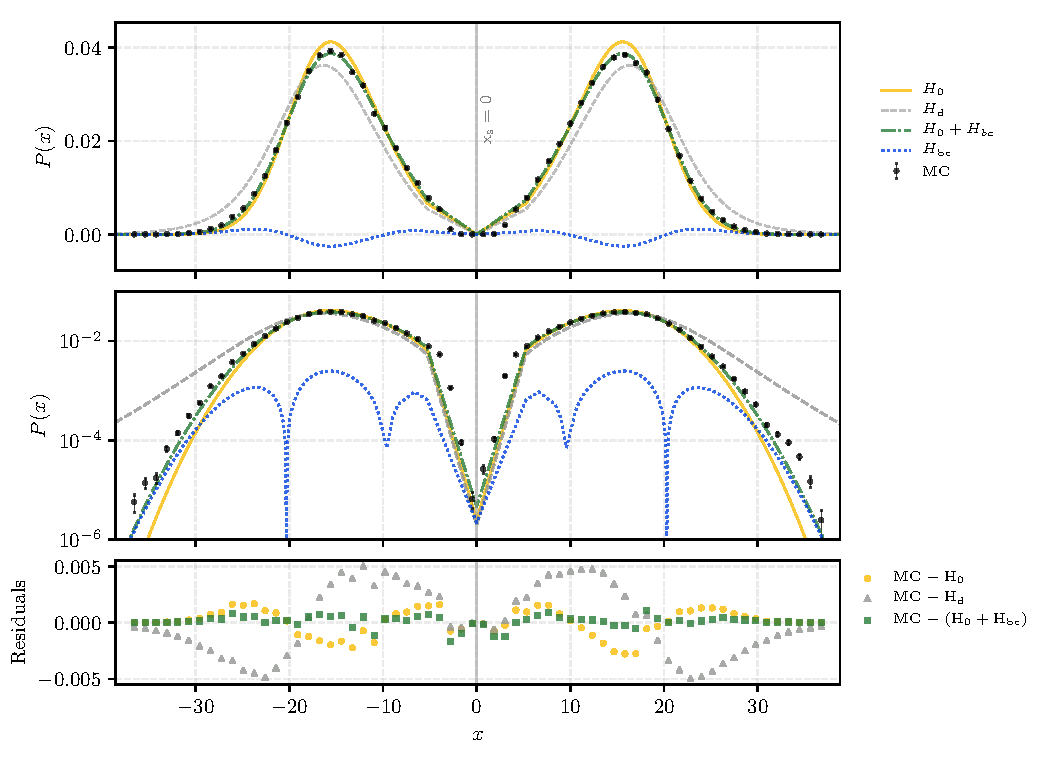
\includegraphics{final_residual.pdf}
    \caption{Spectrum $P(x)$ vs. frequency $x$. The analytic solutions for the outgoing spectrum are calculated at a line center optical depth of $\tau_0 = 1 \times 10^7$ and $a = 4.72\times 10^{-4}$ with $x_s = 0.0$. The top panel is linear scale, the middle panel is log scale with $|\rm H_{bc}|$ shown instead of $\rm H_{bc}$, and the bottom panel is the residual of each solution with Monte Carlo.} 
    \label{fig:sol_mc_residual_0}
\end{figure}

We now compare each of the previously-discussed solutions for surface flux to the Monte Carlo results. The spectrum $P(x)$ is defined as the specific luminosity at the surface divided by the source luminosity, or
\be \label{eq:prob_spectrum}
P(x) = \frac{16\pi^2R^2H(R, x)\Delta}{L}.
\ee
This is normalized as $\int P(x)dx = 1$. Since $H(r, x)$ is per $d\nu$, a factor of $\Delta$ gives the expression the correct units. 

In Figure \ref{fig:sol_mc_residual_0}, the Monte Carlo escape probability as a function of frequency is shown along with that of the solutions $H_{\rm d}$, $H_0$, and $H_{\rm 0 + bc} = H_0 + H_{\rm bc}$ for an optical depth of $\tau_0 = 10^7$ and photons emitted at line center $\rm x_s = 0$.  The $H_{\rm bc}$ term is negative at the peak of the spectrum and positive in the line wing such that, when added to $H_0$, it corrects for the apparent excess of flux in the peaks of the spectrum. The solution with the correct frequency-dependent boundary condition enforced, $H_{0 + \rm bc}$, has lower residuals to Monte Carlo results than the other solutions, especially in the line wing. The boundary term corrects the deficit of $H_0$ in the line wings, further improving agreement with the numerical result. Note that the residuals to the $H_0$ solution are a close match to the $H_{\rm bc}$ term, since the Monte Carlo represents the ``true'' solution, $H$, and $H_{\rm bc} = H - H_0$. It is evident that the divergent solution $H_{\rm d}$ fails in the line wings.

 \begin{figure}
    \centering
    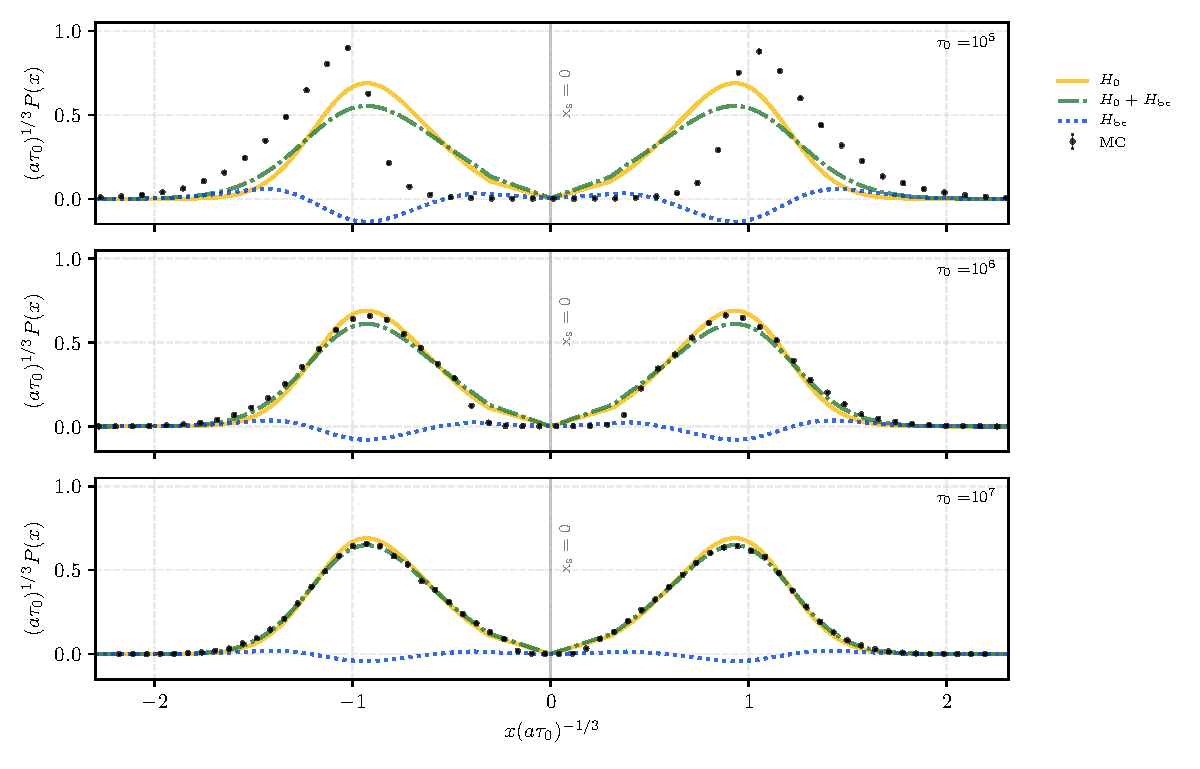
\includegraphics{tau_threepanel.pdf}
    \caption{The same as Figure \ref{fig:sol_mc_residual_0}, but for $\tau_0 = 10^5, 10^6, 10^7$. The $x$ and $y$ axes are scaled by $(a\tau_0)^{1/3}$. Photons are initialized with $\rm x_s = 0.0$ in each case.}
    \label{fig:sol_mc_tau}
\end{figure}

The size of $H_{\rm bc}$ is dependent on $\tau_0$. $H_{\rm bc}$ is significant even at $\tau_0 {\sim} 10^7$ where the $H_0$ solution is expected to perform well, i.e., photons are pushed further out into the wing where the simplifying assumptions made in the derivation of the differential equation are a better approximation. 

In Figure \ref{fig:sol_mc_tau} we show the solutions alongside Monte Carlo for $\tau_0=10^5, 10^6$, and $10^7$. From Eq. \ref{eq:hbc_scaling}, the size of the term $H_{\rm bc}$ should become smaller with larger optical depths, following a $(a\tau_0)^{-1/3}$ scaling. Indeed, agreement between Eq. \ref{eq:H0surf} and the Monte Carlo points in Fig. \ref{fig:sol_mc_tau} improves as $\tau_0$ increases, with $H_{\rm bc}$ providing a fractionally smaller correction to $H_0$. One factor of $(a\tau_0)^{1/3}$ has been scaled out of the x-axis such that the peaks of the distributions are horizontally aligned. This scaling has also been applied to the y-axis to preserve normalization of the escape probability. At lower $\tau_0$, the scattering of photons within the Doppler core of the line becomes important, but our analytic solution does not include this effect. The effects of line core scattering can be seen in the Monte Carlo data for $\tau_0=10^5$ and, to a lesser extent, $
\tau_0=10^6$.
 
 \begin{figure}
    \centering
    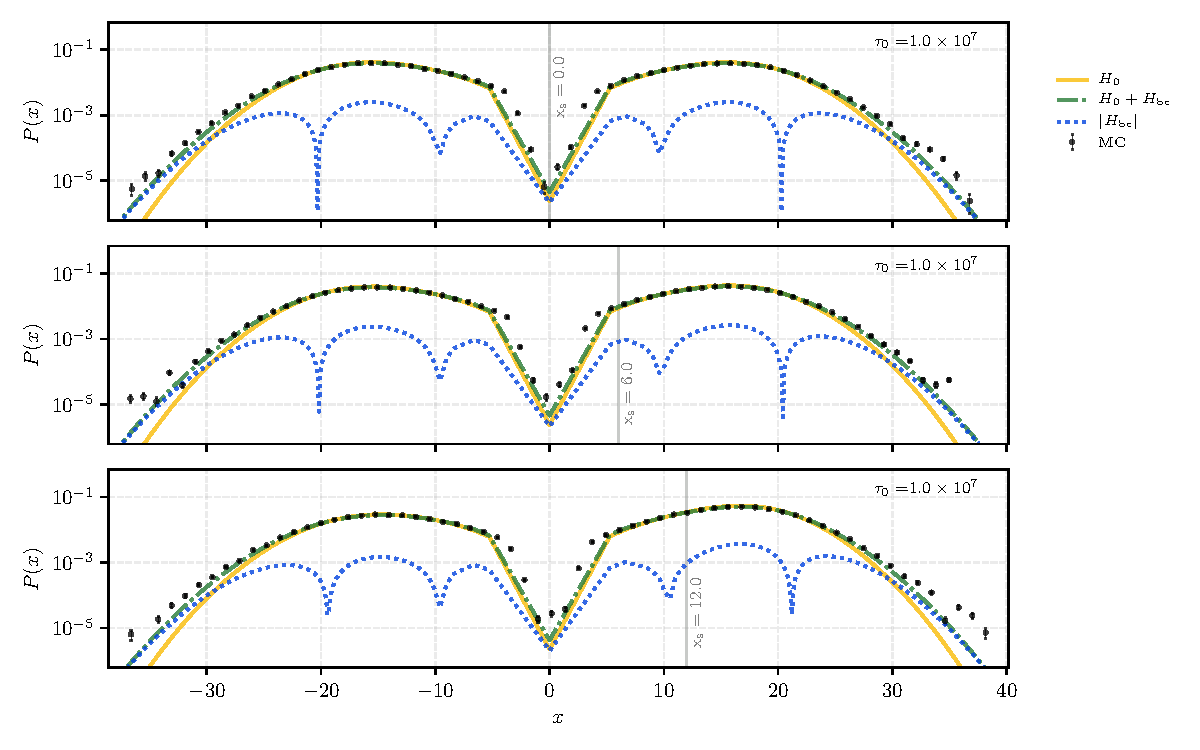
\includegraphics{xinit_threepanel.pdf}
    \caption{The same as Figure \ref{fig:sol_mc_residual_0}, but for $\rm x_s = 0.0, 6.0, 12.0$. The optical depth at each of these source frequencies is $\tau_s = 10^7, 77,$ and $19$, respectively.} 
    \label{fig:sol_mc_xinit}
\end{figure}

 \begin{figure}
    \centering
    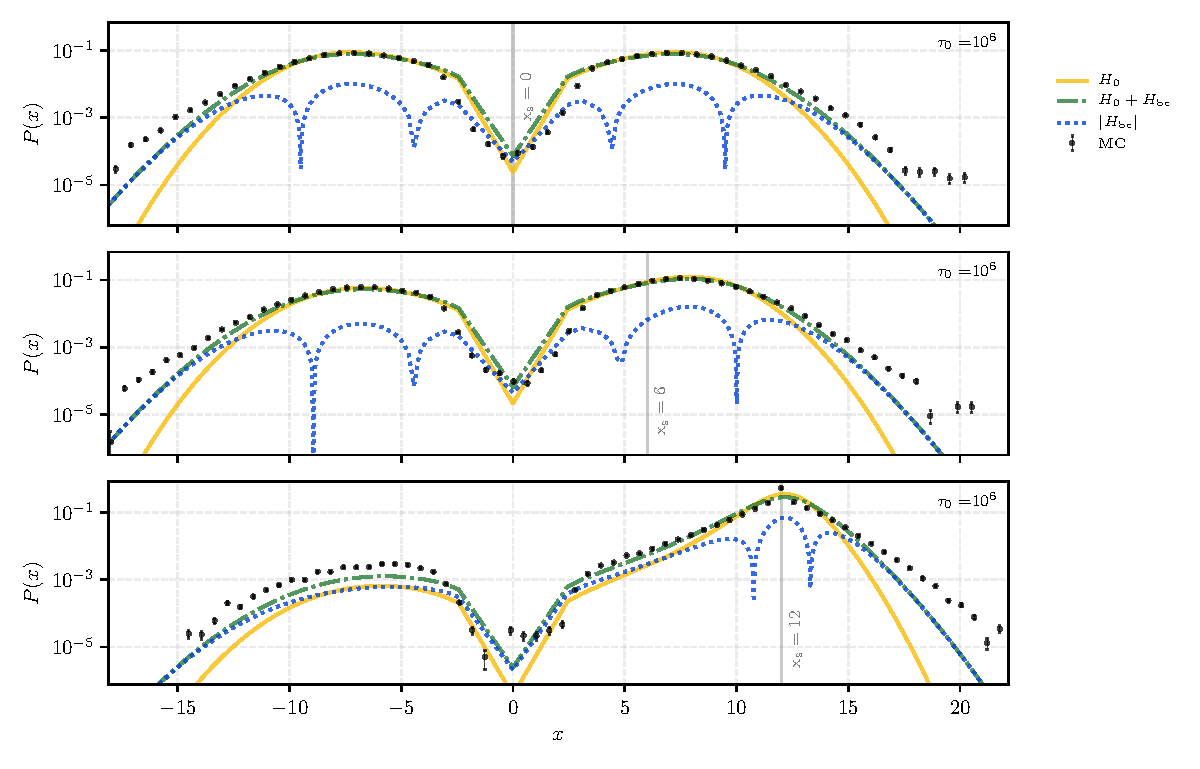
\includegraphics{xinit_threepanel_tau1e6.pdf}
    \caption{The same as Fig. \ref{fig:sol_mc_xinit}, but at a lower optical depth $\tau_0 = 10^6$. The shift $x_s$ is a much larger fraction of the distance to the spectral peak $(a\tau_0)^{1/3}$, and thus the asymmetry in the spectrum is much larger. The optical depth at the source frequency is $\tau_s = 10^6$, $7.7$, and $1.9$ for $x_s=0.0, 6.0,$ and $12.0$, respectively. } 
    \label{fig:sol_mc_xinit_lowtau}
\end{figure}

Next, we show $P(x)$ for $x_s \neq 0$. Photons initialized further out in the line wing have larger mean free paths. The larger spatial diffusion implies greater escape probability for these photons. In the limit that $|\rm x_s|$ becomes large, the distribution becomes a delta function at $x_s$ as all photons escape the sphere without scattering. 

Figure \ref{fig:sol_mc_xinit} shows calculations performed for $x_s = 0.0, 6.0$, and $12.0$ and $\tau_0=10^7$. The asymmetry of the spectrum is slight for $\rm x_s = 6.0$ where $\tau(x_s)=77$, but is larger for $\rm x_s=12.0$ outside the line core where $\tau(x_s)=19$. It is seen here that the difference between the Monte Carlo data and $H_0$ becomes larger as $\rm x_s$ increases. Thus, for large $|x_s|$, inclusion of $H_{\rm bc}$ is more important.

Figure \ref{fig:sol_mc_xinit_lowtau} shows emission away from line center at the same values of $x_s$ as in Figure \ref{fig:sol_mc_xinit}, but for $\tau_0=10^6$ rather than $10^7$. The difference between the left and right side of the escaping spectrum is now substantial since $(a\tau_0)^{-1/3}$ increased by a factor of ${\sim}2$. It is clear from the figure that as $x_s$ extends further into the wing, the spectrum becomes more strongly peaked in frequency. Additionally, since the sphere is increasingly optically thin on the wing, we expect there to be a stronger disagreement with the Monte Carlo as the analytic solution assumed large optical depths.

\begin{figure}
    \centering
    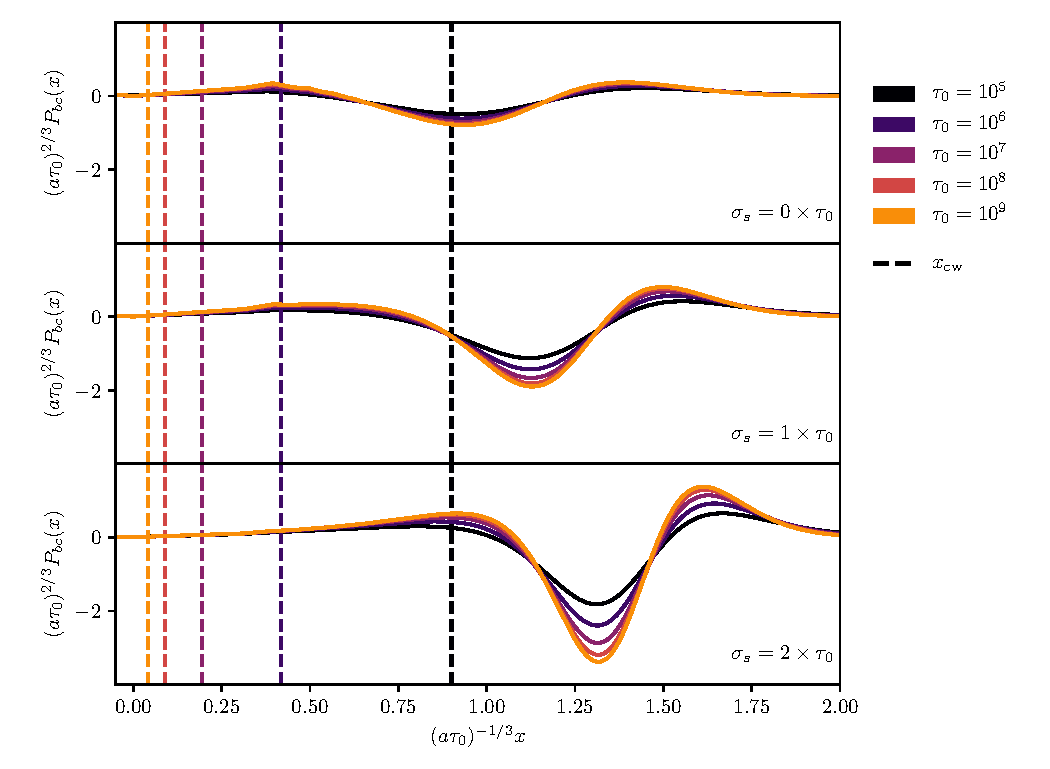
\includegraphics[width=\textwidth]{xinit.pdf}
    \caption{$H_{\rm bc}$ vs. frequency. Here $P(x) = 16\pi^2R^2H_{\rm bc}(R, x)\Delta/L$, as in Eq. \ref{eq:prob_spectrum}. Thicker lines indicate larger optical depth labeled by $\tau_0=10^5, 10^7,$ and $10^9$, and darker lines indicate $\sigma_s$ further from line center, labeled by $\sigma_s=0.0, \tau_0, 2\tau_0$. The location of the core-wing boundary $x_{cw}$ is shown with green vertical lines of increasing thickness for each $\tau_0$. The axes are scaled to show that the size of the corrective factor agrees with the predicted $(a\tau_0)^{-1/3}$ scaling.}
    \label{fig:xinit}
\end{figure}

Figure \ref{fig:xinit} shows how the boundary term $H_{\rm bc}$ scales with both $\tau_0$ and $x_s$. In this figure, $\sigma_s$ is shifted by integer multiples of $\tau_0$ (Eq. \ref{eq:change_of_variables}) such that the source falls near the peak of the spectrum for each $\tau_0$. For clarity, only the $x > 0$ side of the spectrum is shown. From Eq. \ref{eq:hbc_scaling}, it is expected that the fractional size of $H_{\rm bc}$ relative to $H_0$ should become smaller with larger optical depths following $(a\tau_0)^{-1/3}$. This factor has been scaled out of the figure such that solutions for different $\tau_0$ and the same $\sigma_s$ should show close agreement in scale on the figure's vertical axis if the relation holds. Indeed, the scaled solutions converge as $\tau_0$ becomes larger, indicating agreement with the $(a\tau_0)^{-1/3}$ scaling. The remaining discrepancy present in the vertical axis for fixed $\sigma_s$ results from $x_{\rm peak}$ becoming close to $x_{\rm cw}$; at lower $\tau_0$, this causes the line profile approximation in the wing (Eq. \ref{eq:app:line_profile_wing}) to break down. From this, we conclude that the errors introduced by the incorrect separation of variables in \cite{1973MNRAS.162...43H}, \cite{1990ApJ...350..216N}, \cite{2006ApJ...649...14D} and others are indeed proportional to $(a\tau_0)^{-1/3}$.

\section{Time-Dependent Diffusion}
\label{sec:time_dependent}

In order to understand how long it takes for the photons to escape the uniform sphere of gas we must reintroduce the time dependence of the diffusion equation, which was ignored in the steady-state calculations in Section \ref{sec:steadystate}. To obtain the radiative intensity $I=dE/(dAdtd\Omega d\nu)$ on timescales comparable to the light-crossing time $t_{\rm lc} = R/c$, the time-dependent response to a delta function impulse is found. This allows the distribution of photon escape times (the ``wait time distribution'') to be characterized. For simplicity, a $J=0$ boundary condition will be used in the following derivations, which is a rough approximation for $a\tau_0 \gg 1$. 

\subsection{Derivation of the time-dependent solution}
\label{subsec:time_dependent:background}

The emissivity for an impulsive source with energy E, source position $\vec{x}_s$, and frequency $\nu_s$ is derived in Appendix \ref{app:rteqn_derivation}. Considering a photon source at $\vec{x}_s=0$, we have (Eq. \ref{eq:jem})
\be
j_{\rm em} & = & \frac{E}{4\pi} \delta^3(\vec{x}) \delta(\nu-\nu_{\rm s})\delta (t) ,
\label{eq:jem2}
\ee 
The resulting equation for $J(r,\sigma,t)$ is
\be
-3 \frac{k\phi}{c} \frac{\partial J}{\partial t} + \nabla^2 J + \left( \frac{k}{\Delta} \right)^2 \frac{\partial^2 J}{\partial \sigma^2}
& = & - \frac{\sqrt{6} kE}{4\pi \Delta^2} \delta^3(\vec{x}) \delta (\sigma - \sigma_s ) \delta (t).
\label{eq:diffusion_eqn}
\ee
We employ an expansion in terms of spherical Bessel functions in $r$ and Fourier transform in time. The expansion for $J(r, \sigma, t)$ is then
\be
\label{eq:jrsigmat_expansion}
J(r, \sigma, t) = \sum_{n=1}^{\infty} \int_{-\infty}^\infty \frac{d\omega}{2\pi} e^{-i\omega t} j_0\left(\kappa_n r\right) J(n, \sigma, \omega),
\ee
with
\be \label{eq:jnsigmaomega}
J(n, \sigma, \omega) = \frac{2\kappa_n^2}{R} \int_0^R dr\ r^2 j_0(\kappa_n r) \int_{-\infty}^\infty dt\ e^{i\omega t} J(r, \sigma, t).
\ee
Here, $\omega$ describes the time-dependence of $J$. Though it is written as a function of the photon frequency variable $\sigma$, $J(r, \sigma, t)$ is the specific mean intensity $dE/(dA dt d\nu)$ and is a distribution in $\nu$. The Fourier coefficient $J(n, \sigma, \omega)$ has units $dE/(dA d\nu)$. Using Equation \ref{eq:jnsigmaomega}, we obtain
\be \label{eq:diffusion_plugged_in}
 \left( \frac{3k\phi}{c}i\omega  -   \kappa_n^2 \right) J(n,\sigma,\omega)  &+& \left( \frac{k}{\Delta} \right)^2 \frac{\partial^2J(n,\sigma,\omega)}{\partial\sigma^2} = -\frac{2\kappa_n^2}{R} \frac{\sqrt{6}}{4\pi} \frac{kE}{\Delta^2} \frac{1}{4\pi} \delta(\sigma - \sigma_s).
\ee
At $\sigma=\sigma_s$, continuity must be enforced,
\be \label{eq:matching_condition_1}
J(n, \sigma^-, \omega) = J(n, \sigma^+, \omega),
\ee
and the discontinuity in $dJ/d\sigma$ due to the source is
\be \label{eq:matching_condition_2}
\frac{\partial J(n, \sigma^+, \omega)}{\partial \sigma} - \frac{\partial J(n, \sigma^-, \omega)}{\partial \sigma} & = & 
- \frac{\sqrt{6}}{8} n^2 \frac{E}{kR^3}.
\ee
At large values of $\sigma$ the line profile $\phi$ is small and Eq. \ref{eq:diffusion_plugged_in} becomes
\be \label{eq:diffusion_at_large_sigma}
\frac{\partial^2J}{\partial\sigma^2} \approx \frac{\Delta^2\kappa_n^2}{k^2} J,
\ee
which has solutions 
\be
J(n, \sigma, \omega)\ {\sim}\ e^{\pm \Delta \kappa_n \sigma / k}.
\ee
This approximate solution implies a boundary condition at large $|\sigma|$
\be \label{eq:single_j_derivative}
\frac{\partial J}{\partial \sigma} = \mp \frac{\Delta\kappa_n}{k} J,
\ee
where a negative sign is taken for large $+\sigma$ and a positive sign is taken for large $-\sigma$ to chose the finite solution as $|\sigma|\to 0$. Numerical integrations are performed inward toward $\sigma_s$ over several domains: from large $|\sigma|$ to $\sigma_s$, from large $|\sigma|$ to 0, and from 0 to $\sigma_s$, depending on whether $\sigma_s$ is positive or negative. If $\sigma_s=0$, just two integrations are performed inward from large $|\sigma|$ to 0. Initial values for integration are obtained either by setting $J=1$ and $dJ/d\sigma$ from Equation \ref{eq:single_j_derivative} at large $|\sigma|$ or by matching $J$ and $dJ/d\sigma$ at 0. This gives $J$ and $J'$ on either side of $\sigma_s$, where a prime indicates the derivative $\partial/\partial \sigma$. By enforcing the matching conditions Eqs. \ref{eq:matching_condition_1} and \ref{eq:matching_condition_2}, the eigenfunctions $J(n, \sigma, \omega)$ are obtained over the domain of photon frequencies $\sigma$. Since the solutions are linear in the starting conditions, only two integrations with different starting values are necessary.

We now employ an ansatz that roughly agrees with Monte Carlo results for $x_s=0$ based on numerical calculations of this result. However, the analysis presented in Appendix \ref{app:wkb} suggests the ansatz is incomplete in the case where $x_s \neq 0$ and the solution is asymmetric about the line center. Let us define the damping rate to be $\gamma \equiv i\omega$, which is real and positive for damped solutions. At the eigenvalues $\gamma=\gamma_{nm}$, the response $J(n, \sigma, \omega)$ is resonant. Near these $\gamma_{nm}$ poles, the eigenfunctions will have the form 
\be \label{eq:jnsigmaomega_approx}
J(n,\sigma,-i\gamma) & \simeq \frac{ J_{nm}(\sigma) }{\gamma_{nm} - \gamma} + C(\sigma),
\ee
where $C(\sigma)$ varies slowly in $\gamma$. An application of the residue theorem gives
\be
J(r,\sigma,t) & \simeq & j_0(\kappa_n r) J_{nm}(\sigma) e^{-\gamma_{nm}t}.
\ee
Summing over all spatial modes $n$ and over all eigenmodes $m$ for a given $n$, we obtain
\be \label{eq:Jrsigmat}
J(r,\sigma,t) & = & \sum_{n=1}^\infty j_0(\kappa_n r)  \sum_{m=1}^{\infty} J_{nm}(\sigma) e^{-\gamma_{nm}t}.
\ee
This ansatz captures the contributions from $n \times m$ simple poles. Taking a derivative with respect to $r$ and evaluating at the surface $r=R$, we use
\be
\frac{dj_0(\kappa_n r)}{dr} \bigg\rvert_R & =& \frac{d}{dr} \left[ \frac{\sin(\kappa_n r)}{\kappa_n r} \right]\bigg\rvert_R
=  \left( \frac{\cos(\kappa_n R)}{R} - \frac{\sin(\kappa_n R)}{\kappa_n R^2} \right)
\nonumber \\ & = & \frac{(-1)^n}{R}
\ee
to obtain the flux, which is
\be
F(R,\sigma,t) & =& - \frac{4\pi}{3k\phi} \frac{dJ(R,\sigma,t)}{dr} 
= - \frac{4\pi}{3k\phi R}  \sum_{nm} (-1)^n J_{nm}(\sigma) e^{-\gamma_{nm}t}.
\ee
Multiplying by $4\pi R^2$ gives the energy per time per frequency emerging from the sphere to be
\be
\frac{dE}{dtd\nu} & = & - \frac{16\pi^2 R}{3k\phi}  \sum_{nm} (-1)^n J_{nm}(\sigma) e^{-\gamma_{nm}t}.
\label{eq:dEdtdnu}
\ee
Integrating over time yields a factor $1/\gamma_{nm}$, and by integrating over $d\nu$ we find
\be \label{eq:sum_rule}
1 & = &  \sqrt{ \frac{3}{2} } \frac{16\pi^2R\Delta^2}{3kE} \sum_{nm} (-1)^{n+1} \gamma_{nm}^{-1} \int d\sigma J_{nm}(\sigma).
\ee
This non-trivial ``sum rule'' provides a check on the values of $\gamma_{nm}$ and $J_{nm}(\sigma)$. This expression can also be written as
\be
1 & =& \sum_{nm} P_{nm},
\label{eq:sumrule}
\ee
where the contribution of each mode is
\be \label{eq:pnmsoln}
P_{nm} & \equiv & \sqrt{ \frac{3}{2} } \frac{16\pi^2R\Delta^2}{3kE}  (-1)^{n+1} \gamma_{nm}^{-1} \int d\sigma J_{nm}(\sigma).
\ee
These coefficients are negative for odd values of $n$ and positive for even $n$. The size of each contribution scales roughly as $0.5/(m-7/8)^{2/3}$, with a weak dependence on $n$. This indicates the need for a large number of $n$ and $m$ to converge, in that it takes roughly ten times as many $m$ modes to reduce the size of $P_{nm}$ by a factor of ${\sim}$5. 

\subsection{Numerical calculation}

We seek now to calculate the eigenmodes $J_{nm}(\sigma)$ and eigenfrequencies $\gamma_{nm}$ for a given spatial $n$. These will be labelled by an index $m=1, 2, ...$. To measure the size of the response to detect where resonances occur, we sum the absolute value of $J(n,\sigma,-i\gamma)$ over the array $\sigma$. We call this response $f$, and use the index $j$ to represent the value of the response at discrete points $\gamma_j$ over a range of $\gamma$. In places where $f_j > f_{j-1}$ and $f_j>f_{j+1}$, we have bracketed a resonance that occurs in the interval $(\gamma_{j-1},\gamma_{j+1})$. We then hone in on the eigenvalue before continuing the sweep in $\gamma$. To refine the eigenmode solution, we evaluate $f_{j-1}$, $f_j$, and $f_{j+1}$ at the points $(\gamma_{j-1},\gamma_{j},\gamma_{j+1})$. Assuming the form in Equation \ref{eq:jnsigmaomega_approx}, a guess at the correct eigenvalue $\gamma_{nm}$ can be calculated from
\be
\gamma_{\rm guess} &=& \frac{b\gamma_{j-1} - \gamma_{j+1}}{b - 1},
\ee
where
\be
b &=& \left(\frac{f_{j} - f_{j-1}}{f_{j} - f_{j+1}}\right)\left(\frac{\gamma_{j+1}-\gamma_{j}}{\gamma_{j-1}-\gamma_{j}}\right).
\ee
This is repeated by replacing initial points $(\gamma_{j-1},\gamma_{j},\gamma_{j+1})$ with closer estimates while the size of the response grows as the resonance is approached. After iterating an eigenvalue $\gamma_{nm}$ to convergence, we now find the corresponding eigenfunction $J_{nm}(\sigma)$. We can solve for $J_{nm}(\sigma)$ by comparing two points $\gamma_1$ and $\gamma_2$ near the resonance, cancelling $C(\sigma)$ in the difference to find
\be
J_{nm}(\sigma) & \simeq & \frac{ J(n,\sigma,-i\gamma_1)  - J(n,\sigma,-i\gamma_2) }{ 1/(\gamma_{nm}-\gamma_1) - 1/(\gamma_{nm}-\gamma_2)}.
\ee
\begin{figure}
    \centering
    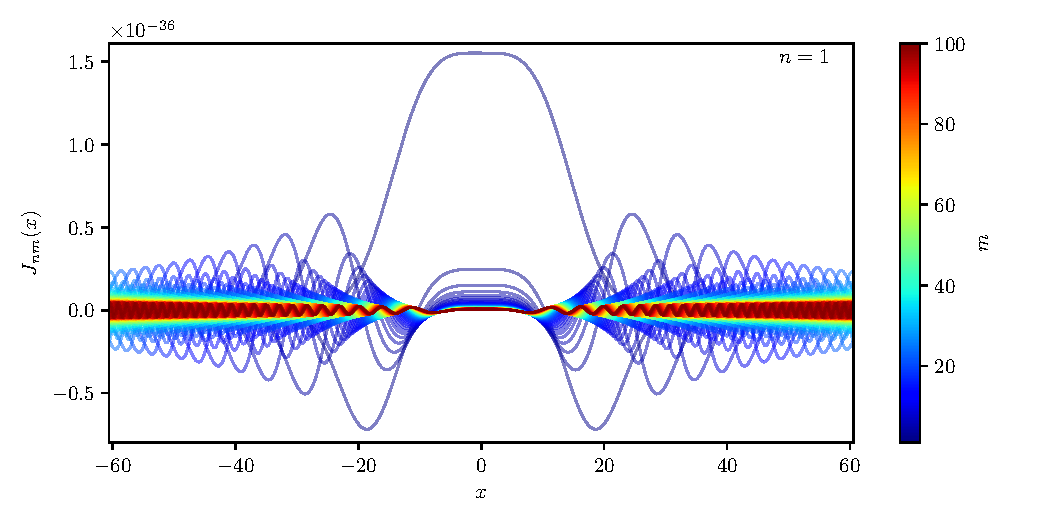
\includegraphics{Jsoln_n1_m100.pdf}
    \caption{Eigenfunctions $J_{nm}(x)$ for the lowest-order spatial eigenmode $n=1$, and $m=1, ..., 100$ with $x_s=0$, $a = 4.72\times 10^{-4}$ and $\tau_0=10^7$.}
    \label{fig:jsoln}
\end{figure}
\noindent The form of a single eigenmode $J_{nm}(\sigma)$ is oscillatory out to some turning point, $\sigma_{tp}$, at which point the function becomes evanescent. The location of the turning point can be found by ignoring the delta-function discontinuity at the source frequency $\sigma_s$ in Eq. \ref{eq:diffusion_plugged_in} and examining the resulting homogeneous differential equation. We obtain
\be \label{eq:wkb_differential_eqn}
\frac{d^2J}{d\sigma^2} & = & \left[ \left( \frac{\kappa_n \Delta }{k} \right)^2 - \frac{3\phi \gamma\Delta^2}{ck}\right] J,
\ee
where the line profile is approximated as in Eq. \ref{eq:app:line_profile_wing}. When the coefficient on the right hand side is positive, exponential growth or decaying evanescent solutions are found. This occurs on the line wings. When the coefficient on the right hand side is negative, oscillatory solutions are found (propagation), which occurs near the line core. The boundary between propagation and evanescence occurs at the turning point, given by
\be \label{eq:sigma_tp}
\sigma_{\rm tp} & = & \sqrt{\frac{2a}{\pi}}\left( \frac{k \gamma}{ \kappa_n^2 c \Delta} \right)^{3/2}
\ee
Thus, to ensure accuracy in each term of Eq. \ref{eq:Jrsigmat}, the bounds of $\sigma$ must be set sufficiently far outside of $\sigma_{\rm tp}$ such that the function is small at the edges. The scale of an $e$-folding in $J_{nm}(\sigma)$ is $k/(\kappa_n \Delta) = \tau_0 / (\sqrt{\pi} n)$, so a grid of $\sigma$ is chosen that spans a large enough number of $e$-foldings that no oscillatory behavior is present at the boundaries of the calculation.

The eigenfunction's oscillatory forms have varying amplitudes which sum to create the final form of the mean intensity. The largest contribution always comes from the ($n=1, m=1$) lowest-order eigenfunction. Fig. \ref{fig:jsoln} shows a set of eigenfunctions $J_{nm}(\sigma)$ to illustrate their relative scales for different $m$ at a fixed spatial eigenmode $n$. The overall scale of the $J_{nm}(\sigma)$ are set by the factor $E/(kR^3)$ with $E$ arbitrarily set to 1, $k = \tau_0 \sqrt{\pi} \Delta / R$, and $R = 10^{11}$ cm. For H atoms with $T=10^4$ K and $\tau_0=10^7$, an eigenfunction has typical size ${\sim} E a / \left(R^2 \Delta \right) = 10^{-37}$. Additional terms add smaller-magnitude, faster-oscillating components that lead to higher accuracy upon summation with the lower-order terms. The oscillations of various modes must cancel, so many modes $m$ and $n$ are required for convergence to the correct solution. 
\begin{figure}
    \centering
    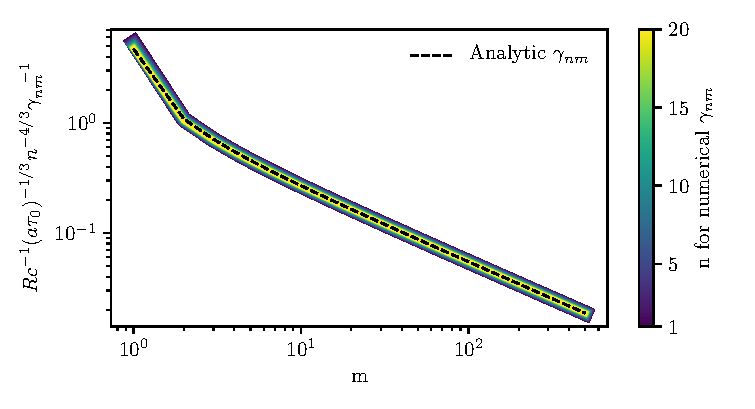
\includegraphics[width=\textwidth]{gamma_nm.pdf}
    \caption{The scaling of numerically-obtained resonant frequencies as compared with the analytic expression in Eq. \ref{eq:gamma_nm}. The data shown is for $\tau_0=10^7$ and $x_s=0.0$.}
    \label{fig:gamma_nm}
\end{figure}
The values of the $\gamma_{nm}$ can be described approximately with Eq. \ref{eq:gamma_nm}. Their values depend on $m$, $n$, and other physical parameters according to 
\be \label{eq:gamma_nm}
\gamma_{nm} = 2^{-1/3} \pi^{13/6} n^{4/3}\left(m-\frac{7}{8}\right)^{2/3}\frac{c}{R}(a\tau_0)^{-1/3}
\ee
as shown in Appendix \ref{app:wkb}. The power law in $m$ is weak, requiring up to $m=500$ to reduce the scale of $\gamma_{nm}^{\ \ -1}$ by two orders of magnitude. When sweeping through to find resonances, Equation \ref{eq:gamma_nm} is used to set the scale of the sweep points $\gamma_j$ to ensure no $\gamma_{nm}$ are missed. The continuity and close agreement with the analytic expression shown in Fig. \ref{fig:gamma_nm} indicate that the numerical solutions are accurate.

\subsection{Comparison with Steady State and Monte Carlo}

We now calculate the distribution of the times it takes each photon to escape the sphere. This is obtained by integrating Eq. \ref{eq:dEdtdnu} over all frequencies. We find
\be
P(t)  & = & \sqrt{\frac{3}{2}} \frac{16\pi^2 R \Delta^2 }{3kE}     \sum_{nm} (-1)^n  e^{-\gamma_{nm}t} \int d\sigma J_{nm}(\sigma) 
\nonumber \\ & = &  \sum_{nm} P_{nm} \gamma_{nm} e^{-\gamma_{nm}t},
\label{eq:waittime}
\ee
which is normalized to unity. For a sufficiently large number of spatial modes $n$ and frequency modes $m$, the result of this sum can agree with Monte Carlo escape time distributions when $x_s=0$, but it is not a fast enough computational method to use as a distribution for sampling. However, the late-time distribution is simply an exponential falloff. The rate constant of the falloff is the lowest-order eigenfrequency, $\gamma_{11}$, and its scale is determined by the coefficient $P_{11}$ as in Eq. \ref{eq:pnmsoln}. Thus, an approximate ``fitting function'' that captures both the peak of the escape time distribution and the exponential falloff is
\be \label{eq:fitting_function}
P(t) = \exp{\left[-\left(\frac{t_{\rm diff}}{t}\right)^2\right]} \times \gamma_{11} P_{11} e^{-\gamma_{11}t}.
\ee
The first term represents the early-time distribution, which then transitions to an exponential falloff past a point $ct_{\rm diff}/R = (a\tau_0)^{1/3}$, where $t_{\rm diff}$ is the characteristic diffusion timescale.

In Fig. \ref{fig:tau_scaling}, it is shown that the time constant of exponential decay in fitted Monte Carlo escape time distributions converges with $\gamma_{11}^{-1}$ at sufficiently high $\tau_0$, following a $t\propto(a\tau_0)^{1/3}$ scaling. At lower $\tau_0$, the effects of line core scattering are most important, leading to a larger discrepancy in the characteristic escape timescale. Here, the Monte Carlo accurately characterizes the photons which scatter in the core many times before escaping, while the semi-analytic solution does not capture this behavior as it uses only the Lorentzian piece of the line profile and does not use enough spatial modes to accurately model the frequency regime near line center. However, as $\tau_0$ grows, the effect of core scattering becomes smaller and the approximations hold, agreeing well with the expected $(a\tau_0)^{1/3}$ scaling for the rate constant.

\begin{figure}
    \centering
    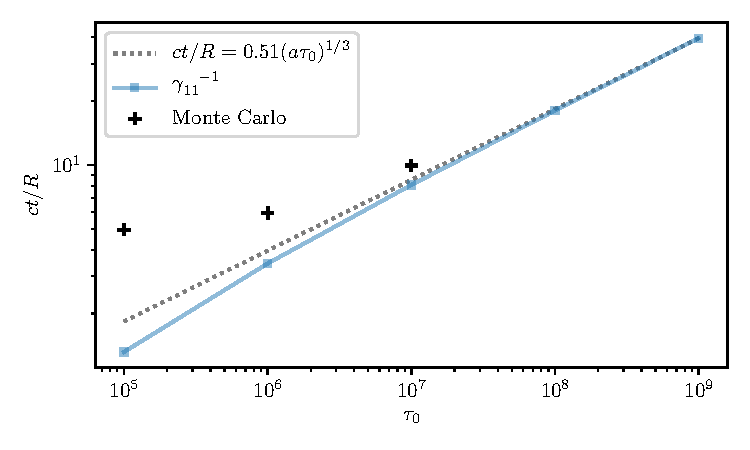
\includegraphics[width=0.75\textwidth]{tau_scaling.pdf}
    \caption{Characteristic timescales as a function of $\tau_0$. $\gamma_{11}^{-1}$ and a fit of the exponential falloff for the Monte Carlo escape time distribution are shown to converge to a $t \propto (a\tau_0)^{1/3}$ scaling at large $\tau_0$. The Monte Carlo points on this figure are obtained by fitting only the exponential piece of the escape time distribution to obtain the rate constant.}
    \label{fig:tau_scaling}
\end{figure}

We now evaluate the time-integrated spectrum of the response to an impulse and compare it with the solution for the $H_0$ steady-state spectrum (Eq. \ref{eq:H0surf}). Integrating Eq. \ref{eq:dEdtdnu} over all times gives a distribution for the emitted frequencies. Dividing by the energy $E$, we find the probability distribution
\be \label{eq:spectrum}
P(\nu) & = &  \frac{16\pi^2 R}{3k\phi E}  \sum_{nm} (-1)^{n+1} \gamma_{nm}^{-1} J_{nm}(\sigma).
\ee
Integrating over $\nu$ then gives unity as required by the sum rule in Eq. \ref{eq:sumrule}. 

In Fig. \ref{fig:steadystate}, the spectrum for $x_s=0$ and $\tau_0=10^7$ is shown for a sum up to $n=20$ and $m=500$ (labelled ``Time-integrated'') as compared with two analytic solutions: the steady state $H_0$ solution with no time dependence (``Steady State'') and the result for summing \textit{only} spatial modes in the eigenfunction expansion with the time dependence ignored (``Partial Sum''), as in Eq. \ref{eq:H0surf}. Additional spatial modes contribute to the solutions' accuracy in the core of the line. If more spatial modes are calculated, the agreement with the steady state spectrum extends further toward the line core, with an infinite number of modes required for convergence at $x=x_s=0$. If additional frequency modes are calculated, faster-oscillating terms are incorporated into the sum over eigenmodes which create more perfect cancellations with the lower-order terms, reducing the ``ringing'' seen in the time-integrated spectrum. Extending the calculation deep into the line core by adding additional spatial modes could have an impact on the accuracy of the escape time distribution, but this would primarily affect the distribution at late times due to the large mean diffusion time of photons near the line core. This was the motivation for choosing a comparatively low number of spatial eigenmodes with respect to the number of frequency eigenmodes calculated.

\begin{figure}
    \centering
    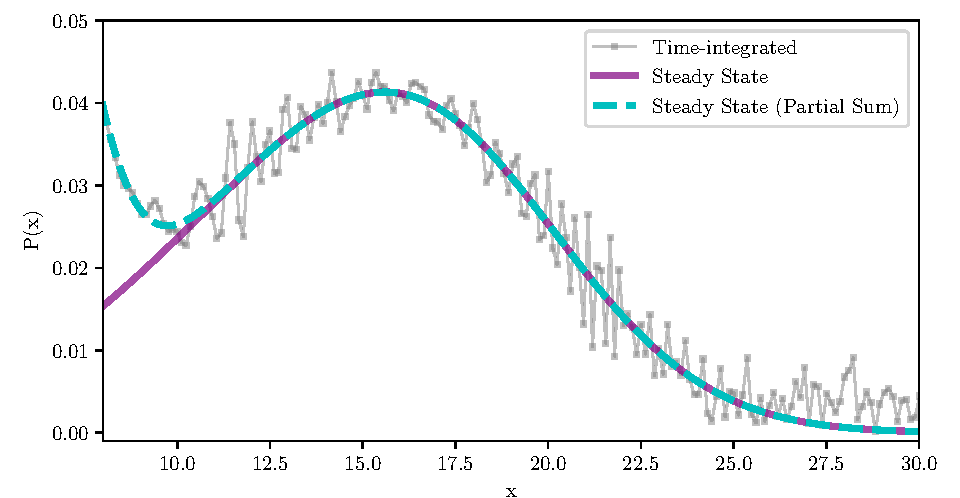
\includegraphics{steadystate.pdf}
    \caption{Comparison of steady-state and time-integrated spectra for $n=1, ..., 20$ and $m=1, ..., 500$ with $x_s=0$, $a = 4.72\times 10^{-4}$ and $\tau_0=10^7$.}
    \label{fig:steadystate}
\end{figure}


In Figure \ref{fig:escape_time} escape time distributions calculated from Eq. \ref{eq:waittime} are shown alongside Monte Carlo and the fitting function Eq. \ref{eq:fitting_function} for $\tau_0=10^6, 10^7$ with $x_s=0$. It is seen that the fitting function matches well with the late-time behavior of the eigenfunction solution, indicating that the tail of the escape time distribution can be modeled effectively by simple exponential decay. The remaining disagreement between the tail of the distribution and the Monte Carlo data is likely due to line core scattering which is not modeled by the eigenfunction solution, but improves for larger optical depth as seen in the figure. A cumulative distribution function can be created from Eq. \ref{eq:fitting_function} using a simple rejection method, which allows the function to be sampled rapidly.

\begin{figure}
    \centering
    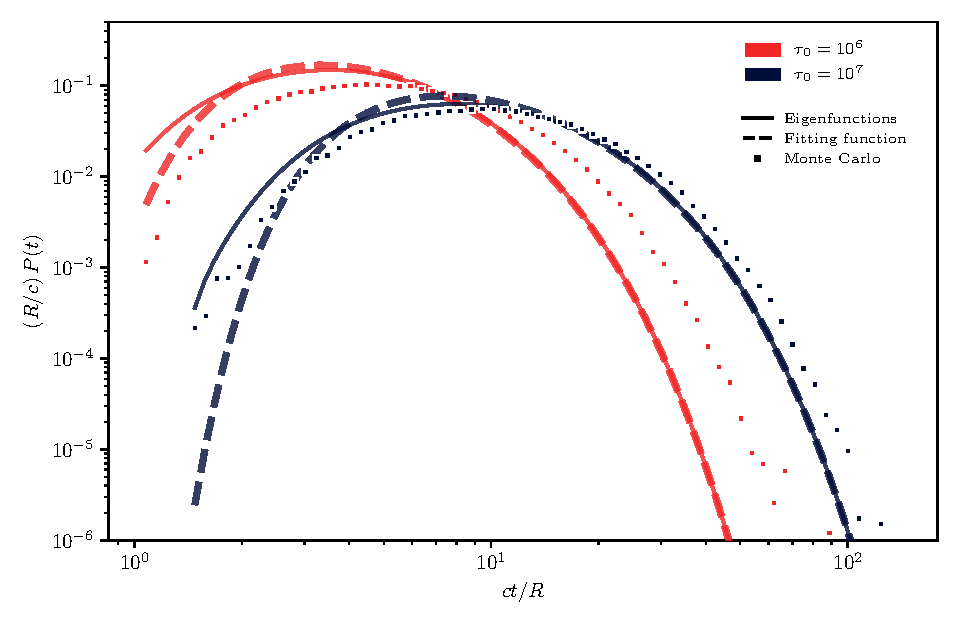
\includegraphics{waittime.pdf}
    \caption{Wait time distributions of escaping photons for $\tau_0=10^6$ and $10^7$, which is fit using Eq. \ref{eq:fitting_function}. A sum over 20 spatial eigenmodes and 500 frequency eigenmodes is labeled ``Eigenfunctions''. All calculations were performed with a monochromatic source of photons at line center ($x_s = 0.0$).}
    \label{fig:escape_time}
\end{figure}

The effect of many scatterings in the Doppler core affects the tail of the escape-time distribution, since photons with frequencies near line center will take longer to escape. This explains the deficit of photons in the semi-analytic escape time distributions at late times, in that the rate constant for the exponential falloff is overestimated slightly as compared with the Monte Carlo. The error in this rate constant is a function of $\tau_0$ since the effect from the Doppler core is greatest when it extends into the peak of the spectrum.

\section{Discussion}

A primary goal of this work is to present a solution for mean intensity ($J$) and flux ($H = F/4\pi$) of photons near line-center frequency $\nu_0$ in a uniform sphere. We have generalized a spherically symmetric solution derived by \cite{2006ApJ...649...14D} (called $H_0$ here) to allow a monochromatic source of photons with frequencies away from line center. We have made a correction to their incorrect $J=0$ surface boundary condition that allows the proper condition $J=\sqrt{3}H$ to be satisfied at the surface of the sphere. This introduces a term $J_{\rm bc}$ which is solved using a continuous Fourier expansion in frequency. Enforcement of the correct boundary term leads naturally to expansion of the spatial dependence in terms of spherical Bessel functions. The continuous expansions are discretized and the Fourier coefficients solved for. The resulting flux correction, $H_{\rm bc}$, scales as $(a\tau_0)^{-1/3}$. Thus, for large $\tau_0$, only a small correction to $H_0$ is needed, while larger errors are present in calculations performed at lower $\tau_0$. Since the Laplacian form of the differential equation is only attainable by approximating the line profile as $\phi \approx a/(\pi x^2)$, our solutions do not model areas where the Doppler core of the \lya line has a significant effect on the scattering of photons. Because the peak of the spectral energy distribution of escaping photons is $x_{\rm peak} = (a\tau_0)^{1/3}$, calculations performed at low $\tau_0$ are inaccurate due to the close proximity of the spectral peak and the Doppler core of the line. This effect is especially prevalent for larger H gas temperature, as the boundary between the Doppler core and line wing extends further out as $T$ increases.

By comparison with Monte Carlo simulations, we have shown that the enforcement of the correct frequency-dependent boundary conditions improves the accuracy of these analytic solutions provided a sufficiently large $\tau_0$. Specifically, this solution shows improvement over previous solutions that utilized the $J=0$ surface boundary condition presented in \cite{1973MNRAS.162...43H} and \cite{1990ApJ...350..216N}. Several papers have previously compared these analytic models to Monte Carlo and seen discrepancies on the order of this correction. For example, in the top-left panel of Figure 1 from \cite{2006ApJ...649...14D}, the \lya spectrum emergent from a sphere of uniform optical depth is shown for $\tau_0=10^5, 10^6,$ and $10^7$ at a temperature of $T=10$ K, corresponding to $a=1.5 \times 10^{-2}$. The dotted line showing their theoretically-derived spectrum (called $H_0$ here) displays an excess at the peak of at least 5-10 percent as compared with the Monte Carlo for $\tau_0=10^5$ and $10^6$. Though our calculations were performed with a higher gas temperature of $T=10^4$ K, we show in Figure \ref{fig:sol_mc_tau} that the excess present in $H_0$ is corrected by our treatment of the boundary condition at $\tau_0 = 10^7$. In \citet{2015MNRAS.449.4336S}, the peak excess in the \lya spectrum is particularly noticeable for line center optical depths of $\tau_0=10^6$ and $10^7$ in the top panel of their Figure 5, which used slab geometry and a gas temperature of $T=10^4$ K. Again, the error in their solution is of order 5-10 percent. $H_{\rm bc}$ is positive in the line wing and negative at the peak of the spectrum, which matches with the discrepancies noted in these solutions. They are too large at the spectral peaks and too small further out in the wing, and the error scales approximately as $(a\tau_0)^{-1/3}$.

The time-dependence of the problem is solved for a $J=0$ boundary condition to characterize the distribution of photon escape times. Solving the differential equation requires a semi-analytic approach, utilizing an expansion in both space and photon frequency. By matching boundary conditions on either side of the photon source frequency $x_s$, the flux at the surface of the sphere is found as a function of $t$ and $\nu$, expressed as a sum over spatial and frequency modes $n$ and $m$, respectively. Calculating additional spatial eigenmodes provides a more accurate model of the physics nearer to line center, but convergence is slow due to each eigenmode's weak dependence on $n$. Additional frequency eigenmodes introduce fast-oscillating terms that improve the accuracy of the sum, as their contributions cancel with components of lower-order terms to better represent the true solution. Integrating the solution over time produces a spectrum that is shown to agree well with the steady-state calculations in Section \ref{sec:steadystate}, provided a sufficient number of terms in the sum. Integrating the solution over frequency leads to a distribution of photon escape times, which can be compared directly with Monte Carlo simulations. The sum over eigenmodes produces an escape-time distribution that broadly captures the behavior shown by Monte Carlo data---a rise at early times, transitioning to exponential decay in the tail of the distribution. It is expected that the accuracy of the rate constant for the tail of the distribution is limited by the effect of the Doppler core, which can trap photons at high optical depths until they diffuse outward in frequency, weighting the distribution toward later times. This physics is not modeled by our solution for two reasons: 1) our calculations ignored the Gaussian component of the Voigt line profile, leaving the Lorentzian piece which is accurate only in the line wing, and 2) knowing the core is not modeled accurately, we do not include a large enough number of spatial eigenmodes in the sum to resolve it. However, an approximate fitting function dependent on parameters $a$ and $\tau_0$ is found that adequately represents the escape time distribution within these constraints.

This leads in to the primary application of this work. Models of the escape of hydrogen gas in exoplanet atmospheres can be constructed with a treatment of resonant scattering of \lya in spherical geometry. The Monte Carlo method can be used for this problem, but is limited by its high computational demand for large $\tau_0$ where there are many photon scatterings before escape. We seek to develop a computationally efficient random walk model which requires a solution in spherical geometry. There are several methods that are commonly used to accelerate Monte Carlo radiation transfer calculations, including core skipping methods \citep{1968ApJ...153..783A,2002ApJ...567..922A} and hybrid diffusion methods \citep{2018MNRAS.479.2065S} but we believe that these methods are not sufficient for our application. Another approach with wide application is modified random walk methods, such as those discussed in \citet{1984JCoPh..54..508F, 2009A&A...497..155M, 2010A&A...520A..70R}; an outgoing photon is randomly sampled on the surface of the outgoing sphere by drawing its properties from distributions in outgoing frequencies, directions, and escape times, based on solutions to the diffusion equation. A method similar to this has been applied by \citet{2006ApJ...645..792T} to Lyman $\alpha$ transfer using the \cite{1990ApJ...350..216N} solution, but this solution of course does not use the correct frequency-dependent boundary condition at the surface of the sphere. Furthermore, to perform a full radiation hydrodynamic simulation with Monte Carlo acceleration, it will be necessary to calculate radiation forces due to \lya transfer on the faces of each grid cell in the simulation. Similar calculations have been done in \citet{1976ApJ...208..286W} in plane-parallel geometry. However, these solutions are limited to optical depths below $2.5 \times 10^3$. For this work, it would be necessary to model line center optical depths of up to 1 million or more. We will utilize the solution derived here as the basis for our own novel implementation of the modified random walk method.

\section{Summary}

We have examined previous solutions to \lya transfer in the limit of large optical depth, noting that the separation of variables and treatment of the boundary condition in \cite{1973MNRAS.162...43H}, \cite{1990ApJ...350..216N}, \cite{2006ApJ...649...14D} and others does not produce a valid solution to the transfer equation. Here, we have derived the solution in spherical geometry with an appropriate treatment of the surface boundary condition, examining the spectral and time dependence of the resulting equations. The key result is that the errors in the previously-cited works have been quantified via a correction term, $H_{\rm bc}$, which resolves an excess in flux at the spectral peak and a deficit in the line wing of the calculated spectrum of \lya radiation as compared with Monte Carlo. The size of $H_{\rm bc}$ is of order unity when the spectral peaks are near the Doppler core, and diminishes at larger $\tau_0$ following a $(a\tau_0)^{-1/3}$ scaling. Introducing time-dependence to the transfer equation leads to another solution which is solved numerically with an eigenfunction expansion. We demonstrate that it agrees with the steady-state spectrum for $x_s=0$ when integrated over time, though its rate of numerical convergence is slow and requires a sum over many modes to become accurate. This treatment is incomplete for emission away from line center ($x_s\neq0$), however, since any terms that would allow asymmetry in the spectrum are not present in the sum. The time-dependent solution is utilized to create wait-time distributions for photons escaping the sphere of optically-thick hydrogen gas, which can be sampled in lieu of traditional Monte Carlo simulations that would be computationally demanding. We compare the calculations from the time-dependent solution with Monte Carlo for a sample of $\tau_0$, noting general agreement in the resulting escape time distributions. In future work, this will be used to accelerate Monte Carlo \lya transfer at large optical depths with potential applications in radiation hydrodynamic simulations of the atmospheres of exoplanets.

\acknowledgments

NASA ATP grant 80NSSC18K0696, ``Exoplanetary MHD Outflows Driven by EUV Heating, Lyman alpha Radiation Forces and Stellar Tides".
\restartappendixnumbering

\appendix
\section{ derivation of the transfer equation } \label{app:rteqn_derivation}

The problem is as follows. The radiative intensity $I = dE/(dA dt d\Omega d\nu)$ is the energy per perpendicular area $dA$, per time $dt$, per solid angle $d\Omega$ and per frequency $d\nu$ \citep{1986rpa..book.....R}. Here the time-dependence of $I$ has been ignored, which assumes the fluid is changing on timescales long compared to a light-crossing time. The intensity $I=I(\vec{x},\vec{n}, \nu)$ will be considered a function of position $\vec{x}$, photon (unit) direction vector $\vec{n}$, and cyclic frequency $\nu$. In the Eddington and two-stream approximations, $I(\vec{x},\nu) \simeq J(\vec{x},\nu) + 3 \vec{n} \cdot \vec{H}(\vec{x},\nu)$, where $J=(1/4\pi) \int d\Omega I$ is the mean intensity and $\vec{F} = 4\pi \vec{H}= \int d\Omega \vec{n} I$ is the flux.  

The transfer equation is \citep{1986rpa..book.....R}
\be
\frac{1}{c} \frac{\partial I}{\partial t} + \vec{n} \cdot \grad I & =& - \left( \alpha_{\rm sc} + \alpha_{\rm abs} \right) I + (1-p) j_{\rm sc} + j_{\rm em}.
\label{eq:rteqn}
\ee
The scattering coefficient, or inverse mean free path to scattering, is 
\be
\alpha_{\rm sc} & = & n_{\rm sc}\, \frac{\pi e^2}{m_e c}\, f\, \frac{\mathcal{H}(x,a)}{\sqrt{\pi} \Delta}
= k \phi.
\ee
The absorption coefficient $\alpha_{\rm abs}$, or inverse mean free path to true absorption, is a sum over number density of the absorber times absorption cross section. Once the incoming photon has promoted the electron to an excited state, the collisional de-excitation probability is $p$, and hence only a fraction $1-p$ of the excitations lead to re-emission of photons. Photon destruction will not be considered, so $p$ is set to 0 in this work.

\citet{1973MNRAS.162...43H} first showed that the transfer equation for the mean  intensity $J$ will satisfy a Poisson equation involving second derivatives of space and frequency variables. In this section we will briefly review the derivation of this equation including photon destruction terms and an emission term.

 ``Hummer Case II-b"  \citep{1962MNRAS.125...21H} will be used for the redistribution function, for which the incoming photon is absorbed by the atom according to the natural broadening in the rest frame, re-emitted with a dipole phase function $g(\vec{n},\vec{n}^\prime)=(3/16\pi)(1+[\vec{n}\cdot \vec{n}^\prime]^2)$, which is appropriate for a 1s-2p transition \citep{1982qe}, and the result is averaged over a Maxwell-Boltzmann distribution of speeds for the atom. The result can be written
\be
j_{\rm sc}(\vec{x},\vec{n},\nu) & = & k \int \frac{ d^3v}{ \pi^{3/2} v_{\rm th}^3} e^{-v^2/v_{\rm th}^2}\, 
\int d\Omega^\prime \int d\nu^\prime \,
g(\vec{n},\vec{n}^\prime) 
\nonumber \\ & \times & 
\delta \left( \nu - \nu^\prime - \nu_0 \vec{v} \cdot (\vec{n}-\vec{n}^\prime)/c \right)
\left( \frac{\Gamma/4\pi^2}{ \left(\nu^\prime - \nu_0 - \nu_0 \vec{v} \cdot \vec{n}^\prime/c \right)^2 + (\Gamma/4\pi)^2 } \right)  \,
I(\vec{x},\vec{n}^\prime,\nu^\prime)
\nonumber \\ & = & 4\pi k \int d\Omega^\prime \int d\nu^\prime R(\vec{n},\nu; \vec{n}^\prime,\nu^\prime) I(\vec{x},\vec{n}^\prime,\nu^\prime),
\ee
which defines the Case II-b redistribution function
\be
R(\vec{n},\nu; \vec{n}^\prime,\nu^\prime) & = & \frac{ g(\vec{n},\vec{n}^\prime) }{ 4\pi }
\int \frac{ d^3v}{ \pi^{3/2} v_{\rm th}^3} e^{-v^2/v_{\rm th}^2}\,
\delta \left( \nu - \nu^\prime - \nu_0 \vec{v} \cdot (\vec{n}-\vec{n}^\prime)/c \right)
\left( \frac{\Gamma/4\pi^2}{ \left(\nu^\prime - \nu_0 - \nu_0 \vec{v} \cdot \vec{n}^\prime/c \right)^2 + (\Gamma/4\pi)^2 } \right)
\ee
found in \citet{1962MNRAS.125...21H}.


The integral of the redistribution function over outgoing and incoming frequency are
\be
\int d\nu\ R(\vec{n},\nu; \vec{n}^\prime,\nu^\prime) 
& = & \frac{1}{4\pi} g(\vec{n},\vec{n}^\prime) \phi(\nu^\prime)
\ee 
and
\be
\int d\nu^\prime \ R(\vec{n},\nu; \vec{n}^\prime,\nu^\prime) 
& = & \frac{1}{4\pi} g(\vec{n},\vec{n}^\prime) \phi(\nu)
\ee 
where the right hand side is the usual Voigt function, the thermal average of the Lorentzian. The former result implies that the integrated source and sink terms for scattering cancel for $p=1$. In addition, $d\nu d\Omega 4\pi R(\vec{n},\nu; \vec{n}^\prime,\nu^\prime)/\phi(\nu^\prime) $ is the normalized distribution for the outgoing $\vec{n}$ and $\nu$ given the incoming $\vec{n}^\prime$ and $\nu^\prime$. 

This probability distribution can be used to define the moments of the frequency shift
\be
\langle \Delta \nu^n \rangle & = & \frac{ \int d\nu^\prime R (\nu-\nu^\prime)^n}{\int d\nu^\prime R}
= \frac{1}{\phi(\nu)}
\int \frac{ d^3v}{ \pi^{3/2} v_{\rm th}^3} e^{-v^2/v_{\rm th}^2}\,
\left( \frac{\nu_0 \vec{v} \cdot (\vec{n}-\vec{n}^\prime) }{c} \right)^n
\left( \frac{\Gamma/4\pi^2}{ \left(\nu - \nu_0 - \nu_0 \vec{v} \cdot \vec{n}/c \right)^2 + (\Gamma/4\pi)^2 } \right),
\ee
which are functions of $\nu$, $\vec{n}$ and $\vec{n}^\prime$. These integrals can be evaluated in terms of the dimensionless moments of the parallel velocity distribution, defined as
\be
\langle u_\parallel^n \rangle(x,a) & = & \frac{a/\pi }{\mathcal{H}(x,a)} \int 
\frac{du_\parallel u_\parallel^n e^{-u_\parallel^2}  }{(x-u_\parallel)^2 + a^2}.
\ee
The end results for the first and second moments are
\be
\langle \Delta \nu \rangle & = & \Delta \langle u_\parallel \rangle \left( 1 - \vec{n} \cdot \vec{n}^\prime \right)
\\
\langle \Delta \nu^2 \rangle & = & \Delta^2 
\left[ \langle u_\parallel^2 \rangle
\left( 1 - \vec{n} \cdot \vec{n}^\prime \right)^2
+ \frac{1}{2} \left( 1 - \left( \vec{n} \cdot \vec{n}^\prime\right)^2 \right) \right].
\ee

For small frequency shifts $\nu-\nu^\prime$, the incoming intensity may be expanded as 
\be
I(\vec{x},\vec{n}^\prime,\nu^\prime) & \simeq  &
I(\vec{x},\vec{n}^\prime,\nu) 
+ 
\frac{\partial I(\vec{x},\vec{n}^\prime,\nu)}{\partial \nu }(\nu^\prime-\nu)
+ \frac{1}{2} \frac{\partial^2 I(\vec{x},\vec{n}^\prime,\nu)}{\partial \nu^2} (\nu^\prime-\nu)^2 + ...
\ee 
and the Fokker-Planck expansion of $j_{\rm sc}$ is
\be
j_{\rm sc}(\vec{x},\vec{n},\nu) & \simeq  & 4\pi k \int d\Omega^\prime \int d\nu^\prime R(\vec{n},\nu; \vec{n}^\prime,\nu^\prime) 
\left[ 
I(\vec{x},\vec{n}^\prime,\nu) + \frac{\partial I(\vec{x},\vec{n}^\prime,\nu)}{\partial \nu }(\nu^\prime-\nu)
+ \frac{1}{2} \frac{\partial^2 I(\vec{x},\vec{n}^\prime,\nu)}{\partial \nu^2 }(\nu^\prime-\nu)^2
\right]
\nonumber \\ 
& =& 
k\phi(\nu) \int d\Omega^\prime g 
\left[ 
I(\vec{x},\vec{n}^\prime,\nu) 
- \frac{\partial I(\vec{x},\vec{n}^\prime,\nu)}{\partial \nu }
\langle \Delta \nu \rangle
+ \frac{1}{2} \frac{\partial^2 I(\vec{x},\vec{n}^\prime,\nu)}{\partial \nu^2 }
\langle \Delta \nu^2 \rangle
\right].
\ee 
To perform the angular integrals, the Eddington approximation for the angular dependence is inserted with the following result
\be
j_{\rm sc} & = & k\phi J - k\phi \Delta \langle u_\parallel \rangle \left( \frac{\partial J}{\partial \nu} - \frac{6}{5} \vec{n} \cdot \frac{\partial \vec{H}}{\partial \nu} \right)
+ \frac{1}{2} \Delta^2 k\phi \left[ 
\frac{\partial^2 J}{\partial \nu^2} \left( \frac{7}{5} \langle u_\parallel^2 \rangle + \frac{3}{10} \right)
- \frac{12}{5} \langle u_\parallel^2 \rangle 
\vec{n} \cdot \frac{\partial^2 \vec{H}}{\partial \nu^2} \right]
\nonumber \\ & \simeq & 
k\phi J - k\phi \Delta \langle u_\parallel \rangle  \frac{\partial J}{\partial \nu} 
+ \frac{1}{2} \Delta^2 k\phi \left( \frac{7}{5} \langle u_\parallel^2 \rangle + \frac{3}{10} \right)
\frac{\partial^2 J}{\partial \nu^2} .
\label{eq:jsc}
\ee
The first term in Eq. \ref{eq:jsc}, $k\phi J$, represents re-emission of the photon through de-excitation of the atom. It cancels the $-k\phi J$ term in Eq. \ref{eq:rteqn} that corresponds to excitation of the atom. The terms involving frequency derivatives of $\vec{H}$, if carried through the calculation, end up giving terms smaller than then largest terms by a factor of $1/x^2$, which is small on the line wing. These terms are ignored from here on.

If only scattering is included, the transfer equation becomes
\be
\frac{1}{c} \frac{\partial }{\partial t} \left( J + 3\vec{n} \cdot \vec{H} \right)
+ \vec{n} \cdot \grad \left( J + 3\vec{n} \cdot \vec{H} \right)
& = & - k\phi \Delta \langle u_\parallel \rangle  \frac{\partial J}{\partial \nu} 
+ \frac{1}{2} \Delta^2 k\phi \left( \frac{7}{5} \langle u_\parallel^2 \rangle + \frac{3}{10} \right)
\frac{\partial^2 J}{\partial \nu^2}.
\ee
Integrating over angle and frequency then gives
\be
\frac{1}{c} \frac{\partial J(\vec{x}) }{\partial t} +  \grad \cdot \vec{H}(\vec{x}) & = & \int d\nu
\left( - k\phi \Delta \langle u_\parallel \rangle  \frac{\partial J}{\partial \nu} 
+ \frac{1}{2} \Delta^2 k\phi \left( \frac{7}{5} \langle u_\parallel^2 \rangle + \frac{3}{10} \right)
\frac{\partial^2 J}{\partial \nu^2}
\right) 
\nonumber \\ & =& 
k \int d\nu J \frac{\partial }{\partial \nu} 
\left( \phi \Delta \langle u_\parallel \rangle
+ \frac{\partial }{\partial \nu}\left[ \frac{1}{2} \phi \Delta^2 
\left( \frac{7}{5} \langle u_\parallel^2 \rangle + \frac{3}{10}  \right) \right]
\right) = 0,
\ee
where $\vec{H}(\vec{x})$ is the frequency integrated flux, and $\grad \cdot \vec{H}(\vec{x})  = 0 $ if there are no sources or sinks of radiation. Integration by parts has been used to factor $J$ out, assuming each term goes to zero at infinity. The quantity inside brackets must be constant, and since each term should go to zero at infinity, that constant is zero. Hence the first and second moments of the frequency shift are related by
\be
\phi \Delta \langle u_\parallel \rangle
& = & -  \frac{\partial }{\partial \nu}\left[ \frac{1}{2} \phi \Delta^2 
\left( \frac{7}{5} \langle u_\parallel^2 \rangle + \frac{3}{10}  \right) 
\right].
\ee
As an example, on the damping wing, the line profile can be approximated as 
\be \label{eq:app:line_profile_wing}
\phi \simeq \frac{a}{\pi x^2 \Delta}
\ee
with $\langle u_\parallel \rangle \simeq 1/x$ and $\langle u_\parallel^2 \rangle \simeq 1/2$, and so this identity is satisfied. The redistribution function can then be rewritten
\be
j_{\rm sc} & \simeq & k\phi J + \frac{1}{2} k \Delta^2 \frac{\partial }{\partial \nu} 
\left[ \phi  \left( \frac{7}{5} \langle u_\parallel^2 \rangle + \frac{3}{10}  \right)\frac{\partial J}{\partial \nu}  \right]
\simeq k\phi J + \frac{1}{2} k \Delta^2 \frac{\partial }{\partial \nu} 
\left( \phi \frac{\partial J}{\partial \nu}  \right),
\ee
where the last equality (see e.g. \citealt{1994ApJ...427..603R}) is valid on the damping wing where $\langle u_\parallel^2 \rangle \simeq 1/2$.
The following equations will use the approximations for the damping wing.

Thus far the transfer equation is
\be
\frac{1}{c} \frac{\partial }{\partial t} \left( J + 3\vec{n} \cdot \vec{H} \right) + \vec{n} \cdot \grad \left( J + 3 \vec{n} \cdot \vec{H} \right)
& =& j_{\rm em}
- \left( k\phi + \alpha_{\rm abs} \right) \left( J + 3 \vec{n} \cdot \vec{H} \right)
+
(1-p) \left[
k\phi J + \frac{1}{2} k \Delta^2 \frac{\partial }{\partial \nu} 
\left( \phi \frac{\partial J}{\partial \nu}  \right)
\right]
\nonumber \\ & \simeq & 
j_{\rm em} - 3k\phi \vec{n} \cdot \vec{H} - \left( p k\phi  + \alpha_{\rm abs} \right) J 
+ \frac{1}{2} k \Delta^2 \frac{\partial }{\partial \nu} 
\left( \phi \frac{\partial J}{\partial \nu}  \right),
\label{eq:rteqn2}
\ee
where leading order dissipative terms were kept in the second equality.
The moment equations are
\be
\frac{1}{c} \frac{\partial J}{\partial t} + \grad \cdot \vec{H} & = & j_{\rm em} 
- \left(p k\phi +  \alpha_{\rm abs} \right) J
+ \frac{1}{2} k \Delta^2 \frac{\partial }{\partial \nu} 
\left( \phi \frac{\partial J}{\partial \nu}  \right)
\ee
and
\be
\frac{1}{c} \frac{\partial \vec{H}}{\partial t} + \frac{1}{3} \grad J & =& - \left( k \phi + \alpha_{\rm abs} \right) \vec{H}.
\ee
The $\partial \vec{H}/\partial t$ term may be dropped for slowly changing sources.
Assuming the coefficients are constant in space, these two equations can be combined together to find
\be
\frac{1}{c} \frac{\partial J}{\partial t} - \frac{1}{3 (k\phi + \alpha_{\rm abs})} \nabla^2 J
& =& j_{\rm em} 
- \left( p k\phi +  \alpha_{\rm abs} \right) J
+ \frac{1}{2} k \Delta^2 \frac{\partial }{\partial \nu} 
\left( \phi \frac{\partial J}{\partial \nu}  \right).
\ee
Making the change of variables to $d\sigma$ using
\be \label{eq:change_of_variables}
d\sigma = \sqrt{\frac{2}{3}}\frac{d\nu}{\phi \Delta^2},
\ee
the equation can be rewritten in the standard form \citep{1973MNRAS.162...43H}
\be
-3 \left( \frac{k\phi + \alpha_{\rm abs}}{c}\right) \frac{\partial J}{\partial t} + \nabla^2 J + \left( \frac{k}{\Delta} \right)^2 \left( 1 + \frac{\alpha_{\rm abs}}{k\phi} \right)\frac{\partial^2 J}{\partial \sigma^2} & = & 
-3 \left( k\phi + \alpha_{\rm abs}\right) j_{\rm em}
+ 3 \left( k\phi + \alpha_{\rm abs}\right) \left( pk\phi + \alpha_{\rm abs}\right) J.
\label{eq:finaleqn}
\ee
    
For emission with luminosity $L$, with a delta function in space $\delta^3(\vec{x} - \vec{x}_s)$ at source position $\vec{x}_s$, a delta function in frequency $\delta(\nu-\nu_{\rm s})$ at source frequency $\nu_{\rm s}$, and isotropic in angles, the emission coefficient is
\be
j_{\rm em} & = & \frac{L}{4\pi} \delta^3(\vec{x} - \vec{x}_s) \delta(\nu-\nu_{\rm s}).
\label{eq:jem}
\ee
Multiplying by a factor $-3k\phi$, as appears in Eq. \ref{eq:finaleqn}, the delta function in $\nu$ becomes a delta function in $\sigma$ of the form
\be
-3k\phi j_{\rm em}  &= & - \frac{ \sqrt{6} kL}{4\pi \Delta^2} \delta^3(\vec{x} - \vec{x}_s) \delta (\sigma - \sigma_{\rm s}),
\label{eq:jem_v2}
\ee
where $\sigma_s = \sigma(\nu_s)$. 

\section{WKB Approximation} \label{app:wkb}

We start with the differential equation Eq. \ref{eq:wkb_differential_eqn}. Near line center, this has two independent solutions which can be written
\be \label{eq:wkb_J}
J(n,\sigma,s) & = & a_1 \left( \frac{\sigma}{\sigma_{\rm tp}} \right)^{1/2} J_{-3/4}\left( k_c \left[ \frac{\sigma}{\sigma_{\rm tp} }\right]^{2/3} \right)
\nonumber \\ &  + &  a_2 \left( \frac{\sigma}{\sigma_{\rm tp}} \right)^{1/2} J_{3/4}\left( k_c \left[ \frac{\sigma}{\sigma_{\rm tp} }\right]^{2/3} \right),
\ee
where $J_\alpha(...)$ are Bessel functions of the first kind, $a_1$ and $a_2$ are normalization constants, $\sigma_{tp}$ is given in Eq. \ref{eq:sigma_tp}, and $k_c=3\kappa_n \Delta \sigma_{\rm tp}/2k$. The solution far from line center is 
\be
J(n,\sigma,s) & = & a_3 \left( \frac{\sigma}{\sigma_{\rm tp}} \right)^{1/6} Ai\left(k_c^{2/3} \left[ \left( \frac{\sigma}{\sigma_{\rm tp}} \right)^{2/3} - 1 \right]\right),
\ee
where $Ai(...)$ is the Airy function of the first kind. Again, $a_3$ is a normalization constant. When $\sigma_s=0$, we can enforce the discontinuity in Eq. \ref{eq:matching_condition_2} to find 
\be \label{eq:a2}
a_2 & = & - \frac{\Gamma(7/4) \sigma_{\rm tp}}{ 2^{1/4} k_c^{3/4}} \frac{6^{1/2}}{8} n^2 \frac{E}{kR^3}.
\ee
The discontinuity sets the value of $a_2$, and the corresponding term in Eq. \ref{eq:wkb_J} is non-resonant. The discontinuity does not set the value of $a_1$ as that solution does not have a term linear in $\sigma$ when the source is at $\sigma_s=0$. When $\sigma_s=0$, we may show that the solutions both near and far from $\sigma=0$ have the same approximate form in terms of sines and cosines where both functions have short-wavelength behavior. Matched asymptotic expansion \citep{1999amms.book.....B} allows us to relate the normalization coefficients $a_1$ and $a_3$. The matching conditions are
\be \label{eq:a1/a2}
\frac{a_1}{a_2} & = & \frac{ \sin \left( \frac{\kappa_n \sigma_{\rm tp} \Delta}{k} + \frac{\pi}{8} \right) }{ \sin \left(  \frac{\kappa_n \sigma_{\rm tp} \Delta}{k} - \frac{\pi}{8} \right) }
\ee
\be \label{eq:a3/a2}
\frac{a_3}{a_2} & = & \frac{ k_c^{-1/3} }{ \sin \left(  \frac{\kappa_n \sigma_{\rm tp} \Delta}{k} - \frac{\pi}{8} \right) }.
\ee
By setting the to denominator of this expression equal to zero and solving it for the eigenfrequency $\gamma_{nm}$ contained in $\sigma_{\rm tp}$, we find the dispersion relation in Eq. \ref{eq:gamma_nm}.

We have applied this approximation for $\sigma_s=0$. In this case, we have obtained Equations \ref{eq:a1/a2} and \ref{eq:a3/a2} which approach infinity near the eigenfrequencies $\gamma_{nm}$, so there will be no contribution from the $a_2$ term in Equation \ref{eq:wkb_J} at these resonant frequencies. We now seek to understand the behavior of the solution when emission is away from line center ($\sigma_s \neq 0$). The eigenfunction expansion in Equation \ref{eq:Jrsigmat} assumed that a closed contour at infinity, bounding an infinite number of simple poles along the real $\gamma$-axis, could be integrated to find that $J(r, \sigma, t)$ is the sum of the residues of the poles contained within the contour. Equation \ref{eq:a2} shows there is an additional contribution unrelated to the eigenfunctions that is non-resonant. In the case where $\sigma_s \neq 0$, this non-resonant piece contributes to the asymmetry of the the solution about line center. When $\sigma_s=0$, however, the solution is symmetric about line center and the non-resonant piece has no contribution except to produce the matching conditions in Equations \ref{eq:a1/a2} and \ref{eq:a3/a2}. Since we have applied the WKB approximation only when $\sigma_s = 0$, the non-resonant piece which allows the outgoing spectrum to be asymmetric is not captured by the methods outlined here.

\bibliography{ref.bib}{}
\bibliographystyle{aasjournal}



\end{document}

